% !TEX program = xelatex
\documentclass[zihao=-4,a4paper]{ctexart}

% ===== 页面设置 =====
\usepackage[top=2.5cm, bottom=2.5cm, left=3cm, right=2.5cm]{geometry}
\usepackage{setspace}
\onehalfspacing

% ===== 段落格式 =====
\setlength{\parindent}{2\ccwd}
\setlength{\parskip}{0pt}

% ===== 图表与代码 =====
\usepackage{graphicx}
\usepackage{float}
\usepackage{booktabs}
\usepackage{longtable}
\usepackage{listings}
\usepackage{xcolor}
\usepackage{caption}
\usepackage{subcaption}
\usepackage{etoolbox}

% ===== 表格内容5号字 =====
\AtBeginEnvironment{tabular}{\zihao{5}}
\AtBeginEnvironment{longtable}{\zihao{5}}

% ===== 图表标题格式 =====
\DeclareCaptionFont{heiti}{\heiti\bfseries}
\DeclareCaptionFont{songti}{\songti}
\captionsetup{
    font=heiti,
    labelfont=heiti,
    textfont=heiti,
    labelsep=quad,
    justification=centering,
    singlelinecheck=false,
}

% ===== 数学 =====
\usepackage{amsmath,amssymb}
\numberwithin{equation}{section}
\renewcommand{\theequation}{\thesection-\arabic{equation}}
\numberwithin{table}{section}
\renewcommand{\thetable}{\thesection-\arabic{table}}
\numberwithin{figure}{section}
\renewcommand{\thefigure}{\thesection-\arabic{figure}}

% ===== 引用格式（上标角标） =====
% ===== 链接 =====
\usepackage[colorlinks=true,linkcolor=black,citecolor=black,urlcolor=black]{hyperref}

% ===== 页眉页脚 =====
\usepackage{fancyhdr}
\pagestyle{fancy}
\fancyhf{}
\fancyfoot[C]{\zihao{-5}\thepage}
\renewcommand{\headrulewidth}{0pt}
\setlength{\headheight}{5pt}
\fancypagestyle{plain}{
    \fancyhf{}
    \fancyfoot[C]{\zihao{-5}\thepage}
    \renewcommand{\headrulewidth}{0pt}
}

% ===== 代码高亮 =====
\lstset{
    basicstyle=\ttfamily\zihao{5},
    numbers=left,
    numberstyle=\tiny,
    frame=single,
    breaklines=true,
    backgroundcolor=\color{gray!5},
    keywordstyle=\color{blue},
    commentstyle=\color{green!40!black},
    stringstyle=\color{red},
    showstringspaces=false,
}

% ===== 标题格式（使用ctexset） =====
\ctexset{
    section = {
        format = \centering\zihao{-2}\heiti\bfseries,
        beforeskip = 24pt plus 3pt minus 2pt,
        afterskip = 18pt plus 2pt minus 1pt,
    },
    subsection = {
        format = \zihao{4}\heiti\bfseries,
        beforeskip = 18pt plus 2pt minus 1pt,
        afterskip = 12pt plus 2pt minus 1pt,
    },
    subsubsection = {
        format = \zihao{-4}\heiti\bfseries,
        beforeskip = 12pt plus 2pt minus 1pt,
        afterskip = 6pt plus 1pt minus 1pt,
    },
}

% ===== 其他 =====
\usepackage{enumitem}
\usepackage{array}
\usepackage{tabularx}
\usepackage{makecell}

\begin{document}

% ==================== 封面 ====================
\begin{titlepage}
\vspace*{1.5cm}
\begin{center}
    {\zihao{-0}\heiti\bfseries 本科毕业设计（论文）}\\[2.5cm]
    {\zihao{2}\heiti\bfseries 个人健康管理智能体的设计与实现}\\[1cm]
    {\zihao{2}\bfseries Design and Implementation of\\a Personal Health Management Agent}\\[2.5cm]
    {\zihao{3}\songti
    \begin{tabular}{rl}
        院\hspace{2.5em}系：& 计算机科学与技术学院 \\[0.6cm]
        专业班级：& 计算机科学与技术2105班 \\[0.6cm]
        姓\hspace{2.5em}名：& 袁立沛 \\[0.6cm]
        学\hspace{2.5em}号：& U202217212 \\[0.6cm]
        指导教师：& 邱德红 \\[2cm]
    \end{tabular}
    }\\[1cm]
    {\zihao{3}\songti 2026年5月8日}
\end{center}
\end{titlepage}

% ==================== 学位论文原创性声明 ====================
\newpage
\section*{学位论文原创性声明}
\addcontentsline{toc}{section}{学位论文原创性声明}

\vspace{1cm}

{\zihao{-4}\songti
本人郑重声明：所呈交的论文是本人在导师的指导下独立进行研究所得的研究成果。除了文中特别加以标注引用的内容外，本论文不包含任何其他个人或集体已经发表或撰写的成果作品。本人完全意识到本声明的法律后果由本人承担。

\vspace{2cm}

\begin{flushright}
学生签名：\hspace{3cm}\\
\vspace{0.5cm}
日\hspace{2em}期：\hspace{1cm}年\hspace{1cm}月\hspace{1cm}日
\end{flushright}
}

\newpage
% ==================== 学位论文版权使用授权书 ====================
\section*{学位论文版权使用授权书}
\addcontentsline{toc}{section}{学位论文版权使用授权书}

\vspace{1cm}

{\zihao{-4}\songti
本学位论文作者完全了解学校有关保障、使用学位论文的规定，同意学校保留并向有关学位论文管理部门或机构送交论文的复印件和电子版，允许论文被查阅和借阅。本人授权省优秀学士学位论文评选将学位论文的全部或部分内容编入有关数据库进行检索，可以采用影印、缩印或扫描等复制手段保存和汇编本学位论文。

\vspace{1cm}

本学位论文属于

\vspace{0.5cm}

1、保密 $\square$，在\rule{1cm}{0.3pt}年解密后适用本授权书。

\vspace{0.3cm}

2、不保密 $\square$。

\vspace{0.3cm}

（请在以上相应方框内打"✓"）

\vspace{2cm}

\begin{flushright}
学生签名：\hspace{3cm}\\
\vspace{0.5cm}
指导教师签名：\hspace{3cm}\\
\vspace{0.5cm}
日\hspace{2em}期：\hspace{1cm}年\hspace{1cm}月\hspace{1cm}日
\end{flushright}
}

% ==================== 摘要 ====================
\newpage
\section*{摘\hspace{2em}要}
\addcontentsline{toc}{section}{摘要}

{\zihao{-4}\songti
中国有超过2.45亿高血压患者，但知晓率仅51.6\%，治疗率45.8\%，控制率更是只有16.8\%——这意味着超过八成患者最终没能把血压管住。现在不少家庭都备了电子血压计，可测完之后呢？多数人看眼数字就过去了，随便记在纸上，没几天就忘了搁哪儿了。就算有认真记录的习惯，对着一串高低起伏的数值，也很难说清楚这些数字到底在告诉自己什么。至于上网搜索健康建议，搜索结果鱼龙混杂，普通人很难分辨真假。

本文做了一个叫HealthAgent的个人健康管理工具，它想解决的事情不复杂：拍照记下血压、打开首页看趋势、遇到困惑问AI。后端用Python的FastAPI框架加SQLite数据库，前端是React配合Ant Design和ECharts搭起来的界面。

OCR模块是全文最有意思的部分，我们试了好几种方案之后发现，通用OCR在血压计屏幕上的识别效果很差——七段数码管那种字体跟通用OCR训练集里的印刷体差异过大。后来我们走了一条双通路的路线：先用本地HOG+SVM分类器判断图片是七段数码管LCD还是标准字体界面——LCD直达VLM做端到端识别，标准字体走百度云通用OCR加X坐标聚类做字段分配。在10张LCD和10张标准字体图片（共60个标注字段）上测试，端到端准确率均达到100.0\%，而纯OCR方案在LCD场景下准确率均不足20\%。智能问诊这一块，我们用12篇医学相关资料建了向量知识库，Prompt中嵌入用户近14天血压概况，同时设置了六条安全限制——不推荐具体药量、不下诊断结论、事实必须标注引用来源等。自动评测脚本验证下来，引用标注、免责声明和剂量安全三项指标都达到了100\%。

测试方面也做了一些工作：后端86个测试用例全部通过，代码覆盖率82\%，前端15个用例也全部通过，TypeScript严格模式下无类型错误。
}

\vspace{1cm}
\noindent{\heiti\bfseries 关键词：}{\songti 健康管理智能体；OCR图像识别；大语言模型；检索增强生成；时序预测}

\newpage
\section*{Abstract}
\addcontentsline{toc}{section}{Abstract}

{\zihao{-4}
China has over 245 million adults with hypertension, yet the numbers drop sharply at each step of care: 51.6\% are aware of their condition, 45.8\% get treated, and a mere 16.8\% achieve control. Home blood pressure monitors are commonplace, but most users lose track after taking a reading — writing numbers on scraps of paper that get lost, staring at a list of values without knowing what the trend means, or searching online only to wade through unreliable advice.

We built HealthAgent to close this gap. The core workflow is straightforward: photograph the monitor screen, check a dashboard that shows your trends, and consult an AI that grounds its answers in medical references. Python FastAPI with SQLite runs the backend; the frontend combines React 18, TypeScript, Ant Design 5, and ECharts.

The OCR component proved to be the most instructive part of this project. General-purpose OCR models perform surprisingly poorly on blood pressure monitor screens — those seven-segment digits bear little resemblance to the printed text found in standard training corpora. After systematic experimentation, we settled on a classification-first dual-pathway design: a local HOG+SVM classifier (sub-millisecond inference, 100\% accuracy on 20 validation images) routes seven-segment LCD images directly to Tongyi Qianwen's vision-language model for end-to-end recognition, while standard-font images take the Baidu Cloud general OCR path with X-coordinate clustering for field assignment. Across ten LCD and ten standard-font images (sixty annotated fields in total), this design achieved 100.0\% end-to-end accuracy on both categories — compared to pure-OCR baselines that scored below 20\% on LCD images. For the health consultation module, twelve curated medical documents were embedded into a vector store. Each query prompt bundles the user's 14-day blood pressure summary alongside retrieved knowledge chunks, with six safety constraints baked into the system instructions — no dosage specifics, no diagnostic conclusions, mandatory source citations, and a required disclaimer on every response. An automated evaluation harness confirmed these three safety metrics at 100\% across ten test questions.

We built a layered test suite for verification: 86 backend tests pass with 82\% line coverage, and 15 frontend tests pass with zero TypeScript strict-mode errors.
}

\vspace{1cm}
\noindent{\bfseries Keywords:} Health Management Agent; OCR Image Recognition; Large Language Model; Retrieval-Augmented Generation; Time Series Prediction

% ==================== 目录 ====================
\newpage
\section*{目\hspace{2em}录}
\addcontentsline{toc}{section}{目录}
\tableofcontents
\clearpage

% ==================== 第1章 绪论 ====================
\section{绪论}

\subsection{研究背景与意义}

过去四十年，中国人的疾病谱变了个样。传染病退居次要位置，取而代之的是高血压、糖尿病这类需要长期管理的慢性病。按照《中国心血管健康与疾病报告2023》\textsuperscript{[11]}的数据，18岁以上成年人里高血压患病率大概是27.9\%——四个成年人里就有一个，算下来全国患者超过2.45亿人，而且越来越多年轻人也开始中招。但真正让人担心的不是患病率有多高，而是控制情况有多差：知道自己有高血压的人只占51.6\%，在治疗的占45.8\%，最终能把血压管住的只有16.8\%。而大量证据已经表明，只要把血压管好，心脑血管出大事的风险就会大幅降低——收缩压每降10 mmHg，主要心血管事件的风险大约降20\%，中风风险降27\%。

电子血压计现在很多家庭都有了，但"测完之后怎么办"这个问题基本没人解决。大多数人的流程是这样的：挽起袖子测一下→瞄一眼屏幕上的数字→心里大概记一下或者找张纸写下来→过几天就全忘了。对老年人来说就更麻烦了——眼睛看不太清那小屏幕，手也没那么灵活，每次测完要拿笔抄下三个数字，本身就是件挺吃力的事。有些高端血压计可以蓝牙连手机App，但各家的数据不互通，换一台设备之前的历史就断了。还有个大问题是，这些App顶多给你画条血压曲线，从来不告诉你这条曲线到底想说什么——某次高了一点要不要紧张？最近少吃了盐是不是真的有效果？用户只能自己猜。

想找专业的人问问也难。网上一搜高血压，出来的内容什么都有，大部分是卖保健品的营销号，普通人根本分不清真假。去医院问医生当然最靠谱，但挂个号排半天队就为了问几个问题，时间和精力成本都不低，在农村和偏远地区就更不用说了。

最近两年，大模型的能力有了显著提升。OCR拍照识别技术已经相当成熟，拍张照就能提取出数字；RAG技术能把大模型的输出约束在可信的医学知识范围内，有效降低幻觉风险；流式输出也让对话体验更接近跟人交流。能不能把这些技术整合起来，做一个操作简单到老年人也能使用、但内核足够专业的家用工具？这正是HealthAgent的出发点。

HealthAgent的核心功能可以概括为三项：拍照记录血压、看图理解趋势、对话获取建议。把这三个环节串起来，就构成了从数据采集到理解分析再到行动决策的完整闭环。

\subsection{国内外研究现状}

\subsubsection{医疗设备屏幕OCR}

OCR的历史不短，20世纪60年代靠模板匹配和人工几何特征起步，90年代统计机器学习上场，适应性上了一个台阶。Tesseract\textsuperscript{[14]}是这条线上的典型——1985年从HP实验室起步，架构大改三次，2006年开源后成为最普及的通用引擎。深度学习进场后，CNN+CTC把场景文本识别拉到了新高度，CRNN+CTC一度是行业标配。2020年后百度PaddleOCR\textsuperscript{[13]}系列走轻量化路线，v4版本通用中英文识别率做到了95\%以上。脉络很清楚：通用场景在持续变好。

但把通用OCR直接用在血压计屏幕识别上，效果显著下降——这是我们在项目初期反复验证后不得不接受的结论，实际测试中发现，问题集中在三个相互叠加的层面。

第一个层面是显示字体的特殊性。家用血压计基本都是七段数码管或低分辨率LCD屏幕。数码管中"1"的短横容易被认成字母"l"，"8"的两个环形区域在边缘模糊时被错认成"0"或"B"。LCD屏幕上"6"和"5"的笔画一旦出现细微断裂，整体识别结果就会出错。这里有一个值得注意的细节：我们在不同光照条件下对同一台血压计拍摄了多组照片，同一数值在不同照片中的笔画完整性差异相当明显——上午自然光下的"8"清晰可辨，晚上台灯侧光下同一个"8"的上半环就几乎断开了。我们使用PaddleOCR PP-OCRv4\textsuperscript{[13]}和百度云OCR在10张真实的血压计屏幕照片（30个标注字段）上进行了测试，四种纯OCR方案的准确率均不足20\%（PaddleOCR 16.7\%--20.0\%，百度云3.3\%--16.7\%）。排查后确认，根本原因在于模型的训练数据中几乎没有包含七段数码管这类字体样本——这种字体在通用OCR的训练语料中占比极低，导致"1"被错认为"l"、"8"被错认为"0"等系统性的字形误判。

第二个层面是拍摄条件缺乏可控性。用户拍摄时角度、光照条件各异，反光、阴影、手抖导致的模糊等情况都会出现。这跟文档扫描场景里平整、均匀光照的条件完全不一样。我们在内部测试时尝试让几位同学用各自的手机随意拍摄同一台血压计，得到的照片在亮度、角度、清晰度上差异远超预期——有的照片屏幕区域只占画面的不到六分之一。

第三个层面是屏幕信息的混淆问题——屏幕上除收缩压、舒张压、心率之外，还包含时间戳、电池图标、记忆编号等辅助元素。系统不仅要完成字符识别，还要区分哪些数值是目标读数、哪些是无关信息。

三个问题单独分析都有应对思路，但叠加之后构成了一个典型的小样本工程困境：场景过窄导致缺乏现成数据集，数据不足导致模型泛化困难，泛化困难又使每个新样本都成为困难样本。坦白说，我们最初低估了这三个因素相互强化的程度——直到反复试验后才发现，光靠调整单个环节没法从根本上改善整体识别效果。

现有方案大致分为两条技术路线，各自有局限。

传统OCR引擎（Tesseract\textsuperscript{[14]}、PaddleOCR\textsuperscript{[13]}）优势是速度快、成本低，但面对七段数码管这类非标准字体时性能明显下降。Tesseract的LSTM识别层经过大量合成数据训练，对字体变形有一定适应能力，但数码管字体与训练数据的分布差异过大，光靠调整参数很难有效弥补。另一条路线是多模态视觉大模型——GPT-4V\textsuperscript{[5]}、通义千问VL、Gemini Pro Vision等不仅识别数字形态，还会结合屏幕整体布局和字段间空间关系做综合判断，鲁棒性显著增强。但代价同样明显：单次调用2至3秒，API单价达到专用OCR的数十倍，血压测量在理想情况下需要每天做，按这个频率使用VLM的年度费用会远超设备本身成本。

我们最终选择了分类先行的双通路方案：本地HOG+SVM分类器先判断图片类型——七段数码管LCD图片直达VLM做端到端识别（跳过OCR这一步），标准字体图片走百度云通用OCR加X坐标聚类完成字段分配。这套方案的核心洞察是"分类决定路径，而非在一条路径上堆叠模型"——既然已知OCR在LCD场景下注定失败、在标准字体场景下完全胜任，最好的设计不是在OCR后面加兜底，而是在OCR前面加一个分岔口。这种"分类先行、各自为路"的架构在工业界尚不多见，把它引入家用医疗屏幕识别这一细分场景并提供定量对比数据，或许可以视为本文一个微小但有据可查的贡献。

\subsubsection{健康数据趋势分析}

面向个人的健康数据管理工具，国内外近年来涌现出多款产品，各自的定位侧重有所不同。

Apple Health的核心思路是聚合——通过HealthKit把iPhone、Apple Watch和第三方设备数据汇总到一起，覆盖心率、血压、血氧、睡眠等数十项指标。但它的优势在数据汇聚而不是数据解读：系统可以展示"上个月平均收缩压135 mmHg"这样的汇总，但不会进一步解释它的临床含义或给出后续行动建议。Google Fit在2022年改版后引入了WHO\textsuperscript{[12]}和AHA的运动指南作为活动目标参考，在慢性病指标的持续跟踪上同样没做深入。硬件厂商方案的生态绑定更加突出——Omron Connect只兼容欧姆龙蓝牙血压计，更换设备就会导致数据断裂。Withings Health Mate采用多品类策略，覆盖血压计、体重秤、手表等设备，生活方式建议比较细致，但中文适配和国内本地化不足，服务器放在海外，数据同步延迟明显。

国内方面，华为运动健康和小米健康各自拥有大量穿戴设备用户基础。华为在血压管理领域与多家医疗机构开展了合作研究，部分型号手表已支持腕式血压测量和血压健康研究计划，这一"被动测量"的设计思路有实用价值——用户日常佩戴手表就能自动积累数据，不用专门用上臂式血压计进行主动测量。小米健康则通过与小爱同学的语音整合降低了操作门槛，对不熟悉手机操作的老年人群体更加友好。不过整体上，这些平台的重心仍然集中在数据采集与可视化层面，在数据解读方面普遍比较薄弱——通常只提供"本月血压偏高次数：X次"等简单统计，缺乏针对个人情况的趋势分析，也不会主动给出健康建议。用户拿到的是数据，不是判断。

学术界在血压趋势预测上的探索主要有三个方向，各有各的适用边界。

Prophet\textsuperscript{[15]}是Facebook在2017年开源的，它把时间序列拆成趋势、周期和节假日效应三部分分别建模，对缺失值和异常值不太敏感，在家庭场景采样不规律的条件下这确实是个优点。但Prophet至少需要两个完整周期的数据（通常90天以上）才能稳定估计周期参数，新用户或测量不规律的用户到不了这个门槛。LSTM靠门控机制抓长程依赖，在ICU患者生命体征预测这类医疗时序任务上表现很好，但那基于密集采样数据。家庭用户的自测记录通常只有几十条到几百条，单独训LSTM必然过拟合，跨用户训又面临隐私保护和个体差异的双重障碍。ARIMA\textsuperscript{[16]}经典、理论扎实、结果好解释，但它假设序列平稳。真实的家庭血压数据——特别是开始用药或改变生活方式那段时间——几乎一定不平稳，差分、定阶这些前处理步骤对缺乏统计背景的用户门槛不低。

三种方法在家庭场景下面对同一个瓶颈：模型需要足够数据才能输出可靠预测，真实家庭血压数据恰恰是稀疏且不规律的。2022年JMIR一篇系统综述回顾了39项面向消费者的血压管理App研究，结论指出"绝大多数应用仅提供数据可视化，不到15\%的应用有任何形式的预测或趋势分析功能"。我们项目启动前的竞品调研也印证了这一判断。基于此，系统设计原则确定为：数据不足以支撑可靠预测时，明确告知用户"还需要继续测量"，同时完整呈现当前可用的统计信息；数据积累充分后，再提供有统计意义的趋势判断。后文介绍的趋势判定算法即按照"先确保不误导、再争取提供帮助"的原则设计。

\subsubsection{大模型在医疗领域的应用}

大语言模型在医疗健康领域是近两年最活跃的方向之一。2022年底ChatGPT让公众第一次直观感受到AI回答医学问题的能力——虽然早期的回答质量参差不齐，但"对话式问诊"这种交互形态本身已经足够有冲击力。学术界的探索其实更早就开始了。

2018年Google在BERT\textsuperscript{[3]}基础上用生物医学文献继续预训练。做出了BioBERT和PubMedBERT。在命名实体识别、关系抽取等NLP任务上都刷新了当时的记录。但这两个模型的输出形式限定了它们的应用范围——只能做分类和抽取，不能生成自由文本，没法直接用在对话式问诊上。2020年GPT-3\textsuperscript{[4]}的出现改变了这一局面。它在零样本和少样本条件下的泛化表现超出了许多人的预期。模型内部沉淀的医学常识量也相当可观。到2023年7月，Google和DeepMind发布了Med-PaLM 2\textsuperscript{[8]}。在USMLE类问题上准确率达到86.5\%，已经接近执业医师考试水平。相比前代版本，它在回答一致性、事实准确性和安全性上都有明显改进。虽然在真实临床环境中的表现距离"可用"还有距离。中文领域同样进展迅速。HuatuoGPT基于中文医学对话数据做微调，在知识问答和医患对话模拟上取得了良好表现。BenTsao（本草）专攻中医药知识和中西医结合问答。填补了通用模型在中医药领域的空白。

但多项研究也同时指出了三个无法回避的问题。

首先是幻觉问题。大模型有一种让人不太放心的能力——用特别笃定的语气输出完全错误的信息。日常对话中说错一两句影响有限，但在医疗场景下，一条错误的药物剂量建议可能带来实实在在的健康风险。Stanford HAI在2024年发布的医疗AI可信度评估报告中指出，就算是目前表现最好的模型，在医学事实上还有3--5\%的错误率。更值得警惕的是，这些错误集中出现在模型表现得最"自信"的回答里——用户光凭自己的判断几乎识别不了这些错误。

其次是知识时效性问题。模型的知识在训练完成那一刻就冻结了，此后发布的新指南、新证据都没法知道。一个具体的例子是：2024年发布的《中国高血压防治指南》\textsuperscript{[10]}修订版在血压分级标准和用药推荐上都做出了重要调整，但训练语料截止到2022或2023年的模型对此完全无知，还是会按旧版标准回答用户的问题。

第三个问题是缺乏个性化能力。通用模型的"经验"来自海量文本的统计平均——它天然倾向于给出普适性建议，很难结合特定用户的血压历史、年龄、性别、合并症等信息做差异化判断。一名25岁的健康个体与一名70岁伴有糖尿病的老年患者，两者的安全血压范围可能相差10--15 mmHg，但通用模型在对话中很少能敏锐地做出这种区分。模型识别的是统计意义上的"平均人"，而不是眼前具体的对话者。

Lewis等人\textsuperscript{[1]}在2020年NeurIPS上提出了检索增强生成（RAG），为上述三个问题提供了一条工程上可行且成本可控的解决路径。核心思路并不复杂：每次回答问题之前，先从知识库检索与用户问题最相关的文档片段，把这些片段连同系统指令和用户数据组装成Prompt，一起送入大模型。这相当于在每次对话前给模型做一次"临时知识注入"——模型不需要在训练阶段记住所有医学信息，推理时"读一遍"检索到的材料就能回答。RAG抑制幻觉的原理在于让模型输出受限于可验证的外部知识边界，解决时效性靠知识库随时更新而不用重训模型，个性化则靠把用户自己的血压数据嵌入Prompt来实现。同一个问题，不同用户的Prompt中嵌入了不同的14天血压概况，模型给出的回答自然就有了针对性。

跟微调模型比起来，RAG在工程上有几个很实际的好处：改知识只需要更新文档，不用重训模型；每一条事实性陈述都能回溯到知识库里的具体来源——这对医疗场景的价值很明显；部署成本也远低于维护一套定制微调模型的GPU集群。2023年以来，LangChain和LlamaIndex这些RAG编排框架快速成熟，已经在企业知识问答、法律文书检索、医疗咨询辅助等多个场景落地。但这些框架的抽象层级偏高，随之而来的代价是Prompt结构无法完全受控，Token消耗也不够透明——对一个需要精确定义安全边界的医疗AI系统来说，这些是实质性的短板。基于这些考虑，我们决定自行实现RAG的编排逻辑，这增加了代码量，但换来了对安全约束的精确控制——在医疗场景下，这一取舍是合理的。

\subsection{本文的主要工作}

本文的工作围绕几条主线展开，各条线上的时间投入并不均匀——OCR模块所占用的精力最多，原因会在第四章详细说。

在OCR模块上，我们搭了一套分类先行的双通路识别方案。本地HOG+SVM分类器先判断图片是七段数码管LCD屏幕还是标准字体界面——LCD直达通义千问VLM做端到端识别，标准字体走百度云通用OCR加X坐标聚类做字段分配。另一个关键设计是，识别结果不直接入库，而是先回填到前端表单供用户逐字段核对修改，确认没问题了再写入。在健康场景下，一个被认错的数字比一个没认出来的数字更危险，让用户做最终把关是更稳妥的选择。

第二块工作是面向安全的个性化RAG问诊。用12篇医学知识文档构建了向量知识库（向量存储和检索基于sqlite-vec扩展实现），Prompt中嵌入两块动态信息——用户最近14天的血压概况和检索到的知识库片段。系统指令中内嵌了六条安全红线：禁止推荐具体药物剂量、禁止下诊断结论、事实必须标注引用来源、每条回复必须附带免责声明等。我们编写了一套自动评测脚本，每次修改Prompt后可以快速重新验证安全指标，不用靠人工逐条审查——这个脚本在迭代过程中发挥了重要作用，后文会详细说明。

第三块是端到端的数据链路——从采集、趋势分析到可视化看板。包括用户级数据隔离、按数据量自适应调整窗口的趋势判定算法，以及基于ECharts的双Y轴时序看板。

测试这边建了从单元、集成到端到端的分层体系。后端86个测试用例全部通过，代码覆盖率82\%，前端15个用例也全部通过，TypeScript严格模式没有任何类型错误。

\subsection{论文组织结构}

本文后续章节的安排是：第二章说用到哪些关键技术以及为什么选它们；第三章做需求分析和系统架构设计；第四章讲三个核心模块具体怎么实现的；第五章是测试策略和评测结果；第六章总结一下做了什么、还有哪些地方可以接着做。

% ==================== 第2章 相关技术 ====================
\clearpage
\section{相关技术}

这一章介绍HealthAgent用到的几项核心技术。和常规综述不太一样，我不会只罗列技术概念，而是同时说明在这个系统里为什么选了它、没选别的——每个选择背后都有具体的场景约束。

\subsection{光学字符识别技术}

OCR模块的设计经历了从简单串联到分类先行的演进。最终架构分为五步：图像类型分类、路径路由、图像预处理、文本检测与识别、后处理。

在图像预处理环节，输入图像（支持JPG/PNG/WebP三种格式）先转成RGB数组，随后按长边等比缩放到最长不超过1920像素，在保留足够细节的前提下控制文件大小；接着转灰度图降维度，最后用CLAHE（限制对比度自适应直方图均衡化）增强局部对比度。CLAHE把图像划分成8×8个子块，每个子块内独立做均衡化，再通过双线性插值平滑拼接回原图，同时设置对比度上限（clip limit=2.0）防止噪声被过度放大。实测表明，引入CLAHE对缓解屏幕反光和光照不均问题有显著改善。

在文本检测与识别环节，非LCD路径上我们使用百度云通用OCR接口（accurate接口），它对标准印刷字体有极高的检出率，返回结果中每个文字都带有归一化的边界框和置信度。之所以选云端API而非全本地部署，是因为测试发现PaddleOCR\textsuperscript{[13]}在七段数码管LCD场景下的识别效果很不理想（准确率仅16.7\%--20.0\%），且本地GPU推理耗时较长。LCD路径上则直接调用通义千问VLM做端到端识别——实验已证明这是目前应对七段数码管字形的最有效手段。

在后处理与字段分配环节，OCR返回的是一组未排序的识别结果，需要从中筛选出收缩压、舒张压、心率三个数值，同时排除时间戳、电池图标等干扰项。处理规则有四条：首先按边界框高度筛掉明显太小的字（辅助信息比血压读数小得多）；其次优先尝试X坐标聚类——将X坐标相近的token归为"主列"（收缩压+舒张压），X坐标明显偏离的token识别为"侧栏"（心率），聚类不满足条件时回退到Y坐标排序；然后用生理合理范围做数值校验（收缩压60--250、舒张压30--160、心率30--200 mmHg/bpm）；最后用"收缩压必须严格大于舒张压"这一医学常识做一致性检查。经过这四步过滤，大部分噪声信息能被有效排除，字段分配的准确率在标准字体图片上达到100\%。

\subsection{大语言模型与RAG}

大语言模型底层是Transformer\textsuperscript{[2]}解码器架构，通过在海量文本上做自回归预训练来学习语言理解和生成。生成是逐Token自回归的——每一步根据上文算下一个Token的概率分布，再按一定策略采样。我们选的是通义千问的qwen-plus，理由比较务实：接口兼容OpenAI格式，以后切换模型成本低；中文医学术语覆盖得不错；原生支持流式输出；毕设期间有免费额度。

但把通用大模型直接用在医疗场景下有一个绕不开的问题——幻觉。模型会用斩钉截铁的语气说出完全不正确的内容。日常聊天说错一两句不算什么，但在医疗场景下，一条错误的药物剂量建议真的可能带来严重后果。这不是一个可以"以后再说"的问题。

RAG为这个问题提供了一条可行的出路。它的思路不复杂：每次对话时，先拿用户问题去知识库里检索，把最相关的文档片段找出来，然后把这些片段和系统指令、用户数据拼成完整的Prompt发给大模型，模型推理时"读一下"相关资料就能回答，不需要在训练阶段记住所有知识。RAG的核心价值在于：每条回答都能追溯到知识库里的具体文档来源，幻觉风险因此被控制在一个可验证的边界内；知识库更新后不需要重训模型。

我们没有用LangChain这类现成的编排框架，而是自己写了RAG的编排逻辑。主要考虑几个方面：Prompt模板的每一行都能完全掌控，六条安全红线可以逐条审计验证，不会被框架的默认行为悄悄改掉；Token消耗一目了然，不会被框架黑盒吞掉；少引入一堆第三方依赖也意味着少了一堆潜在的兼容性问题和安全漏洞。代价是多写了些代码，但换来了安全层面的确定性——在医疗场景下，这笔交换是值得的。

\subsection{时序数据分析方法}

血压趋势判定上，我们走了轻量路线——滑动平均配合线性回归，没上复杂模型。这个取舍的出发点很现实：家庭场景下的血压数据量通常非常有限。新用户可能只有寥寥几条记录，老用户也不一定天天测，采样间隔完全随缘。在这种数据条件下，复杂模型不仅发挥不了优势，反而可能产出看起来很"确定"实际上不可靠的结果。

滑动平均（SMA）大概是所有平滑方法里最朴素的一个——取固定大小的窗口在序列上滑过去，对窗口内的值求算术平均。好处很明显：计算量小，结果任何人都能看懂。在滑动平均的基础上用线性回归拟合趋势线，斜率的正负和绝对值大小就能大致反映血压的整体走向——往上走、往下走，还是原地踏步。

Prophet\textsuperscript{[15]}和LSTM在学术界各有各的用武之地，但它们都假设你手上有成百上千个数据点。这个前提在家庭自测场景下根本不成立。Prophet需要至少90天的连续序列才能可靠地估计周期参数；LSTM在几十条数据上做训练，得到的结果往往还不如一个简单滑动平均来得稳定——模型越复杂，小样本下的方差问题越严重。基于这些考虑，我们在整个系统中坚持一条原则：数据够了就给趋势判断，数据不够就坦诚告知用户"还需要继续测量"，绝不强行输出一个统计上站不住脚的预测。

\subsection{系统实现技术栈}

后端用的Python 3.11加FastAPI。为什么选FastAPI？我们在Flask、Django和FastAPI之间比较了一下。Flask很轻很灵活，但它的函数视图在项目大了之后要靠Flask-RESTful这些扩展才能自动校验请求参数，类型安全基本靠自觉。Django什么都有——ORM、管理后台、认证系统全自带，但对这个项目来说反而太重了，我们不需要模板引擎（前端是独立React应用），也不需要管理后台。FastAPI刚好夹在中间：靠Python类型注解和Pydantic v2自动生成请求校验、序列化和API文档，同时原生支持async/await——这对需要同时等百度云OCR和DashScope大模型返回的场景确实有用。

数据库选了SQLite，通过SQLAlchemy 2.0 ORM操作。很多人觉得SQLite是"玩具数据库"，但在单机部署场景下它其实是个很务实的选择。MySQL和PostgreSQL需要独立的服务进程——安装、配置、权限管理、日常运维每样都有门槛，这跟"面向普通家庭、部署简单"的目标是对着干的。SQLite整个数据库就是一个文件，不需要任何服务进程，备份只要复制文件；而且支持WAL模式，读写并发性能在家庭场景下绰绰有余。更关键的是sqlite-vec向量扩展——能把向量数据和关系数据放在同一个数据库文件里管理，省去了Elasticsearch或Pinecone那种外部向量数据库的部署和同步麻烦。向量存储用的是sqlite-vec的vec0虚拟表，支持L2距离和余弦距离，1024维的文本嵌入向量建了索引后单次Top-5查询一般在几十毫秒内完成。

前端选择了React 18配合TypeScript。客观来说，Vue 3的Composition API对新手更加友好，模板语法也更贴近传统Web开发，Angular则提供了完整的企业级方案，但框架本身的体量较大。最终选React主要是因为两点：Ant Design 5和ECharts在React生态中的封装最成熟；TypeScript的类型推导在React+hooks模式下支持得最好。组件库用了Ant Design 5——它的ConfigProvider主题定制机制可以在全局统一设Design Token（颜色、圆角、字号、间距等），以后想调整整体视觉风格只需要改一个地方，20多种预置组件覆盖了系统需要的各种界面元素。数据可视化用的是ECharts的echarts-for-react封装，血压看板的双Y轴折线图（左轴mmHg、右轴bpm）加三色异常值标注就是基于它做的。跟D3.js需要手写几十行SVG操作代码比起来，ECharts的声明式配置让可视化的开发轻了不少。

安全认证用了JWT双Token：Access Token 15分钟有效，用来做日常接口鉴权；Refresh Token 7天有效，用来做无感续期。做成两个Token而不是一个长有效期的，主要是想在安全和体验之间取个平衡——如果只用一个长期Token，泄露了整个账户就暴露了；短周期Access Token能把泄露的影响窗口控制在15分钟以内。密码用bcrypt哈希存（cost factor=12），这个参数在安全和登录延迟之间折了个中——cost factor为12时单次哈希大约250ms，暴力破解的成本就被推到了不现实的程度。

% ==================== 第3章 需求分析与系统设计 ====================
\clearpage
\section{需求分析与系统设计}

\subsection{功能需求}

按照毕设任务书的要求，系统要覆盖图像识别、数据管理、智能问诊三块能力，经过梳理最终定了七个功能需求。首先是用户注册与认证，支持用户名和邮箱注册，密码登录后返回JWT双Token，用户可以维护个人资料（昵称、性别、年龄），改密码要验证当前密码，Token过期了通过Refresh Token静默续期，用户不用反复登录。其次是血压计图像OCR识别，用户上传血压计屏幕照片（支持JPG/PNG/WebP，上限10MB），系统自动识别收缩压、舒张压、心率三项，识别结果用彩色Tag标完整度（绿色=三项全了、黄色=缺一两项、红色=一个没认出来），数值自动填回前端表单让用户逐字段确认或修改。在录入方式上，除了拍照录入也提供独立的手动录入入口，OCR的结果先填回表单、用户确认后再写入数据库——这条"机器先认、人来把关"的闭环是系统设计的一个核心理念。在数据展示方面，首页看板聚合展示近期血压均值、最高值、最低值和超标记录数，配一张ECharts双Y轴时序折线图（收缩压/舒张压在左mmHg轴、心率在右bpm轴），支持7天/30天/90天窗口切换。趋势判定上，基于自适应窗口的滑动平均算法给出短期趋势（上升/下降/平稳），数据不够3天的时候直接标"数据不足"，不强行做判断。在智能问诊方面，用户在对话界面输入健康问题，系统从知识库里搜相关资料，结合用户近14天血压数据，通过大模型生成个性化回复，回复以SSE流式逐字输出（打字机效果），每条回复标出引用的知识库来源，支持随时取消。此外还有会话管理功能，可以创建多个独立对话、切换会话、看历史消息、删会话，对话记录持久化保存。

\subsection{目标用户与使用场景}

在细化需求之前，先把系统的目标用户想清楚，很多设计选择后面都能说得通。HealthAgent主要面向三类人。最核心的用户群是居家慢病管理的中老年人，典型画像就是55--75岁的原发性高血压患者，家里有电子血压计，每周测2--5次，但没有长期记录的习惯，对手机玩得不太熟，最想要的就是"拍个照就能记下来、点个键就能看到趋势"。对这类用户来说，最核心的需求其实是降低录入的阻力——手动输三个数字（收缩压、舒张压、心率）对年轻人就是几秒钟的事，但对眼睛花、手指不灵活的老人来说，每次测量后的录入都是一次小小的受挫。第二类是关心父母健康的年轻人，通常25--40岁，跟父母分居两地，父母有高血压或其他慢性病，想了解父母的血压变化趋势，出问题了能及时知道，但不想给父母添太多操作负担——他们往往是App的实际安装者和初始配置人，会帮父母完成第一次设置，同时对"数据共享""家庭组""异常提醒"这些更高级的功能也有明确需求。第三类是高血压初诊或临界人群，典型画像就是体检发现血压偏高（比如130--140/85--90 mmHg）但还没确诊的中青年人，医生建议"在家先监测一段时间看看"。这类人对血压知识了解不多，有各种具体但零碎的问题——"早上测还是晚上测？""测之前能喝咖啡吗？""140算不算高？"——通常也不会为这些问题专门去挂个号，最想要的是打开首页能看到直观的趋势变化，在问诊界面随时能得到靠谱又不吓人的解答。

从这三类人出发，交互上做了几个针对性的选择：OCR拍照作为默认录入方式（降低老人的手动输入成本）；首页看板用彩色卡片和高亮异常值突出关键信息（少看字，多看图）；问诊界面用对话式交互降低学习门槛（不需要懂菜单结构，会打字就行）。

\subsection{非功能需求}

除了功能上的要求，考虑到系统面向的是医疗健康场景，有几条硬性约束必须明确提出来。在性能指标方面，OCR从上传到返回结果不超过3秒——这个数字是估算的，用户在拍照后能接受的等待上限大致如此；问诊首字延迟不超过3秒，如果第一个字超过3秒还没出来，用户很容易认为系统卡死了；看板页面加载1000条记录时首屏渲染不超过1秒；数据库单次查询不超过100ms。这些指标没有经过严格的用户研究校准，主要基于开发过程中的体验判断。在安全与数据隔离方面，所有用户数据严格按user\_id隔离——一个容易被忽略的细节是跨用户访问统一返回HTTP 404而不是403，因为403会暴露"这条记录存在但不属于你"的信息，而404不会，攻击者无法通过状态码差异来枚举系统中的记录；密码经bcrypt哈希后存储，绝不落盘明文；所有业务接口强制通过JWT依赖注入鉴权，不留不需要认证的"调试入口"。在医疗合规约束方面，AI生成的每条回复必须附加免责声明（"以上信息仅供参考，不构成医疗诊断"），模型被禁止输出具体药物的用法用量（这一点没有商量余地），禁止使用确定性诊断语气（如"你患有XX病"），所有事实性陈述必须标注知识库引用来源编号，让用户能看到每条信息的出处。在代码质量标准方面，后端单元测试覆盖率不低于70\%——这个数字不算高，但对于一个需要频繁迭代Prompt和OCR流水线的毕设项目来说，是一个务实的目标；前端TypeScript严格模式零类型错误；全链路E2E测试覆盖核心用户路径。

\subsection{系统架构}

HealthAgent用的是很经典的前后端分离三层架构。

数据层负责持久化存储。关系型数据（用户、血压记录、会话消息）用SQLite通过SQLAlchemy ORM操作，向量数据（知识库文档的嵌入向量）用sqlite-vec扩展的vec0虚拟表存储，两者都放在同一个SQLite文件——不需要单独部署什么中间件，备份也很简单。文件存储（用户上传的血压计照片）直接用本地文件系统，以后如果需要可以换成对象存储。

服务层是业务核心。各个模块职责是分开的：user\_service处理认证和资料管理；ocr\_service编排分类先行的双通路OCR流水线（本地HOG+SVM分类器→LCD直达VLM/非LCD走百度云OCR+X坐标聚类）；bp\_record\_service实现血压记录的增删改查、统计聚合和趋势预测；chat\_service编排RAG全流程（检索→Prompt组装→SSE流式生成）；chat\_store负责会话和消息的持久化。模块之间通过依赖注入传递数据库会话和配置，互相之间耦合不紧。

接口层基于FastAPI对外暴露RESTful API，统一以/api/v1为版本前缀，一共18个端点。接口层的职责包括：用Pydantic Schema校验请求参数、通过Depends依赖注入做JWT鉴权、把服务层的异常统一转成HTTP错误响应。API文档由Swagger UI和ReDoc自动生成。

前端是React单页应用，React Router 6管路由、Zustand管全局状态、Axios做HTTP通信。组件按功能分成页面级（登录、看板、录入、对话等）和通用组件（鉴权守卫、布局框架、错误边界等）。

系统整体架构如图\ref{fig:architecture}所示。

\begin{figure}[H]
\centering
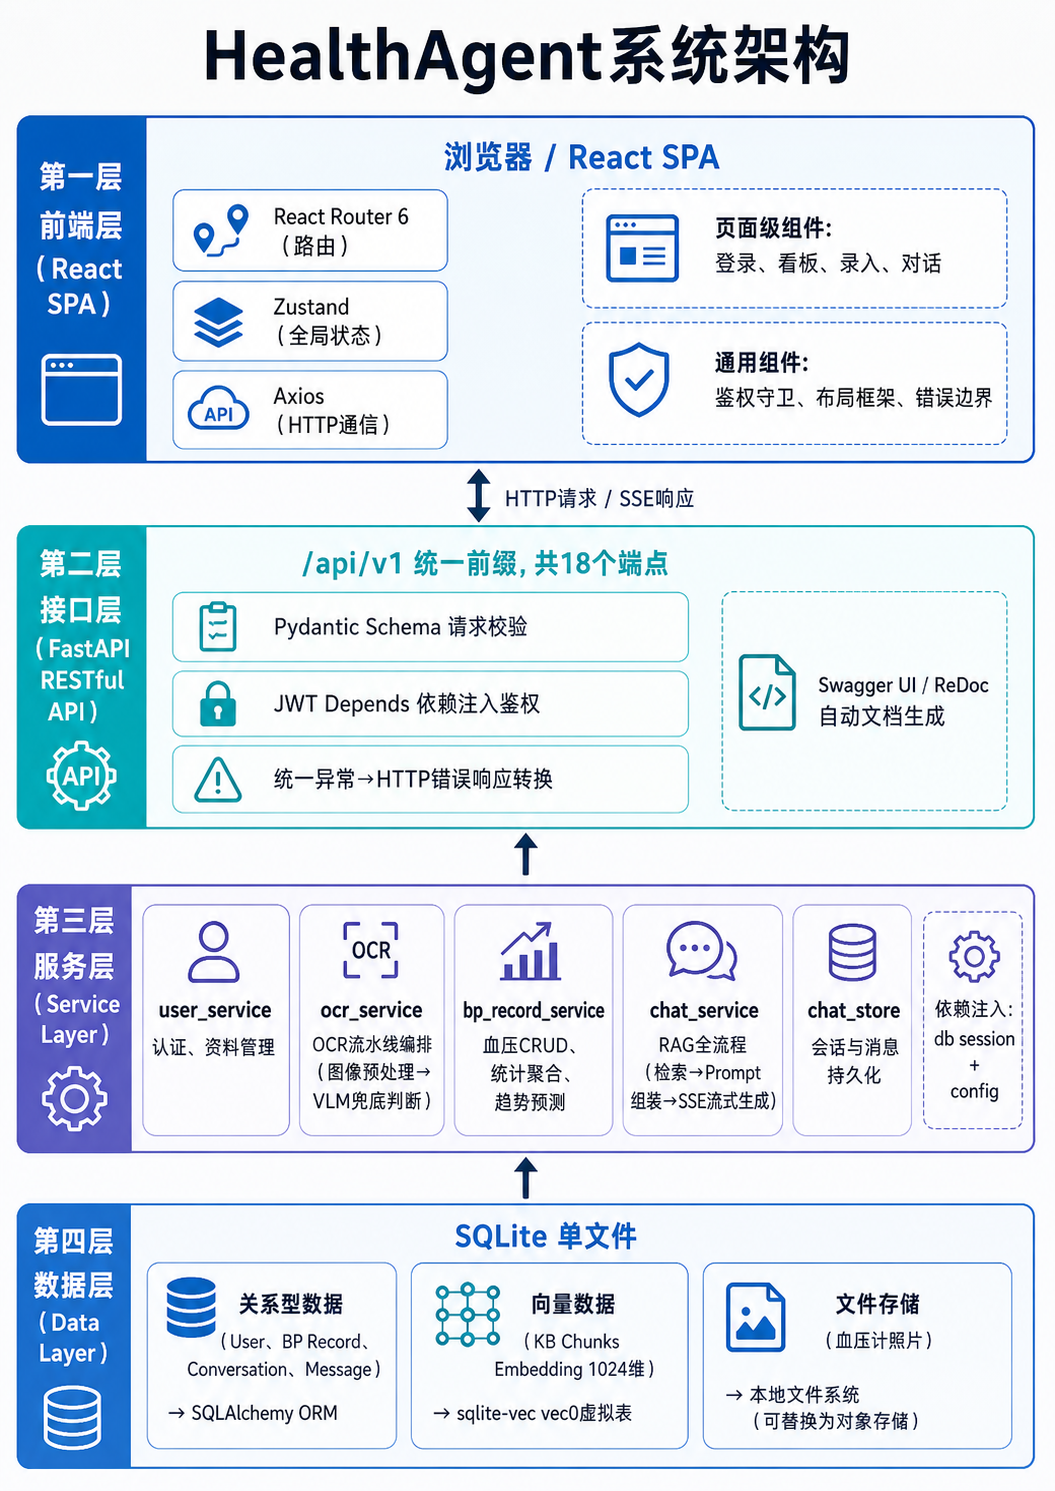
\includegraphics[width=0.5\textwidth]{../pic/pic1.png}
\caption{HealthAgent系统架构}
\label{fig:architecture}
\end{figure}

\subsection{数据库设计}

核心数据库表围绕四组业务对象组织。在用户与认证方面，users表除了存放用户基本信息外，密码经bcrypt哈希后存储，birth\_date字段用来计算年龄——后面做个性化血压阈值判定的差异化建议时，年龄是一个重要输入。在血压记录方面，bp\_records表是系统里读写最频繁的表，measured\_at字段上建了降序索引，因为按时间倒序分页查血压历史是最高频的操作，这个索引对查询性能的影响是决定性的；source字段限定在manual和ocr两个取值；image\_id可以关联回用户上传的原始照片，方便后续怀疑某个数据时溯源确认。在会话与消息方面，conversations和chat\_messages两张表管理问诊对话的全生命周期，chat\_messages中有一个citations\_json列，以JSON数组格式存储每条回答引用的知识库片段详情（chunk编号、所属文档标题、向量距离分数），前端用这个来渲染引用来源卡片——用户点一下就能看到回答参考了哪篇文献的哪个段落。在知识库方面，kb\_documents、kb\_chunks、kb\_vectors三张表构成了知识库的三层存储：kb\_documents用content\_hash做增量去重，内容完全相同的文档不会重复入库，这在文档更新和重复导入时能避免知识库膨胀；kb\_vectors是sqlite-vec扩展提供的vec0虚拟表，存储1024维的文本嵌入向量并维护索引。选择在SQLite内部管理向量数据而非引入独立的向量数据库，主要是为了减少部署复杂度——少一个需要运维的中间件，家庭场景下的系统就更可能被实际用起来。

\subsection{安全设计}

认证安全方面，密码用bcrypt（cost factor=12）做哈希，JWT密钥是随机生成的256位字符串，Access Token有效期15分钟。授权安全方面，所有业务接口通过get\_current\_user依赖注入强制鉴权，服务层对资源归属做二次校验（比记录的user\_id和JWT里的user\_id是不是一致），防止不安全的直接对象引用（IDOR）。数据安全方面，Pydantic输入Schema对所有字段做严格白名单校验，密码字段永远不会出现在任何API序列化输出中，分页查询设了上限防止资源耗尽。

% ==================== 第4章 关键模块实现 ====================
\clearpage
\section{关键模块实现}

本章展开讲三个核心模块的具体实现——这部分涉及大量工程细节，可能是整篇论文里最不"干净"但也最接近实际情况的内容。

\subsection{双通路OCR血压计图像识别}

这是数据采集的入口，也是整个项目里我最花时间折腾的部分。

\subsubsection{整体流水线}

OCR模块的处理流水线一共五个阶段，关键是先分类再选择执行路径。流水线的第一个环节是图像类型分类，使用本地轻量分类器判断图片属于七段数码管LCD血压计屏幕还是其他类型（App截图、电脑看板、打印标签等），分类器基于HOG特征+SVM。HOG特征提取首先计算图像的梯度幅值和方向，对于像素位置$(i,j)$：
\begin{equation}
G_x(i,j)=I(i,j+1)-I(i,j-1),\quad G_y(i,j)=I(i+1,j)-I(i-1,j)
\end{equation}
\begin{equation}
M(i,j)=\sqrt{G_x^2+G_y^2},\quad \theta(i,j)=\arctan(G_y/G_x)
\end{equation}
将图像划分为若干胞元（cell），每个胞元内按梯度方向投票累积为方向直方图，再将相邻胞元组成块（block）做L2归一化后拼接为最终特征向量$\mathbf{x}$。SVM分类器的决策函数为：
\begin{equation}
f(\mathbf{x})=\text{sgn}\Bigl(\sum_{i=1}^{n}\alpha_i y_i K(\mathbf{x}_i,\mathbf{x})+b\Bigr)
\end{equation}
其中核函数选RBF核$K(\mathbf{x}_i,\mathbf{x}_j)=\exp(-\gamma\|\mathbf{x}_i-\mathbf{x}_j\|^2)$。分类器在10张LCD和10张标准字体图像上训练，20张全部正确分类，本地推理耗时不足1毫秒——不产生任何API调用开销，这一步虽然简单但决定了后续整个管线的走向，是双通路架构的路由层。分类完成后进入路径路由：如果分类为LCD，则走LCD直达VLM路径——不再调用百度云OCR（因为实验已经证明OCR在此场景下几乎注定失败，准确率仅3.3\%--16.7\%），直接调用VLM做端到端识别，Prompt包含血压计屏幕识别专用的结构化JSON指令；如果分类为非LCD（App界面、打印标签等），则走OCR主通路——使用百度云通用OCR接口（accurate接口），预处理流程为图像格式标准化→长边等比缩至1920→灰度化→CLAHE对比度增强→Base64编码传至百度云，返回的JSON数组包含识别文字、边界框坐标和置信度，单次调用一般在0.7秒以内。CLAHE（Contrast Limited Adaptive Histogram Equalization）的变换函数为：
\begin{equation}
T(p)=\text{clip}\bigl(H_c(p)\bigr)\cdot\frac{L-1}{N}
\end{equation}
其中$H_c(p)$是经过对比度限幅后的直方图，$L$为灰度级数，$N$为窗口像素数，通过限制局部对比度过度放大的方式来抑制噪声。接下来是结构化字段抽取，OCR返回的结果是杂乱排列的——血压值、时间戳、电池标志、记忆编号全部混在一起，抽取过程分四步进行：首先按边界框高度过滤，设所有OCR识别结果的边界框高度集合为$\{h_1,h_2,\ldots,h_n\}$，中位数为$h_{\text{med}}$，只保留满足以下条件的识别结果：
\begin{equation}
h_i \geq 0.7 \times h_{\text{med}}
\end{equation}
血压读数是屏幕上最大的数字，通常占屏幕高度30--40\%，而时间戳和电池标志的字号明显小得多。；接着按Y坐标排序，把留下的数值按纵坐标从小到大排——家用血压计的屏幕布局很固定，收缩压在上面、舒张压在中间、心率在下面，排好序后按位置分配字段就行；然后做数值范围校验，每个候选值$v$必须满足$v \in [v_{\min}, v_{\max}]$，三个字段的临床合理范围分别为：
\begin{equation}
\mathcal{R}_{\text{sys}}=[60,250],\quad \mathcal{R}_{\text{dia}}=[30,200],\quad \mathcal{R}_{\text{hr}}=[30,220]
\end{equation}
其中收缩压和舒张压单位为mmHg，心率单位为bpm。超范围的值直接当噪声扔掉。；最后做字段一致性校验，若抽取的收缩压$v_{\text{sys}}$和舒张压$v_{\text{dia}}$不满足$v_{\text{sys}} > v_{\text{dia}}$，则丢弃$v_{\text{dia}}$——因为从生理学定义上收缩压必须严格大于舒张压，这个简单的约束能拦掉不少字段归属错误。最后一个环节是VLM兜底复检（仅用于非LCD路径）：在主通路OCR+X坐标聚类完成字段分配后，如果任一必需字段仍为None或一致性校验不通过，会触发VLM做补充识别；不过实测中标准字体图片的OCR数值检出率为100\%，加上X坐标聚类解决了字段互换问题后一致性校验始终通过，因此VLM在此路径上从未被实际触发。这个兜底逻辑仍然保留在代码中，作为极端情况（如照片严重模糊导致OCR完全失败）下的最后一道保险。

\subsubsection{方案对比实验}

我们在10张真实的家用血压计屏幕照片上（含不同光照和屏幕类型），对五种方案做了端到端对比，所有方案均在相同30个标注字段上评估。字段准确率定义为正确识别的字段数与标注字段总数的比值：
\begin{equation}
\text{Accuracy} = \frac{\sum_{i=1}^{N_{\text{fields}}} \mathbb{1}[v_{\text{pred},i} = v_{\text{gt},i}]}{N_{\text{fields}}}
\end{equation}
其中$v_{\text{pred},i}$为预测值，$v_{\text{gt},i}$为标注真值，$\mathbb{1}[\cdot]$为指示函数。结果如表\ref{tab:ocr-compare}所示。

\begin{table}[H]
\centering
\caption{OCR方案对比实验数据（10张LCD屏幕照片，30个标注字段）}
\label{tab:ocr-compare}
\begin{tabular}{lcc}
\toprule
\textbf{方案} & \textbf{字段准确率} & \textbf{平均耗时(s)} \\
\midrule
PaddleOCR PP-OCRv4（CPU，通用中英） & 5/30 (16.7\%) & 1.54 \\
PaddleOCR + CLAHE/反色三变体 & 6/30 (20.0\%) & 1.97 \\
百度云accurate通用OCR & 5/30 (16.7\%) & 0.64 \\
百度云numbers数字OCR + bbox过滤 & 1/30 (3.3\%) & 0.86 \\
\textbf{分类先行双通路（本文方案）} & \textbf{30/30 (100.0\%)} & \textbf{1.00} \\
\bottomrule
\end{tabular}
\end{table}

\begin{figure}[H]
\centering
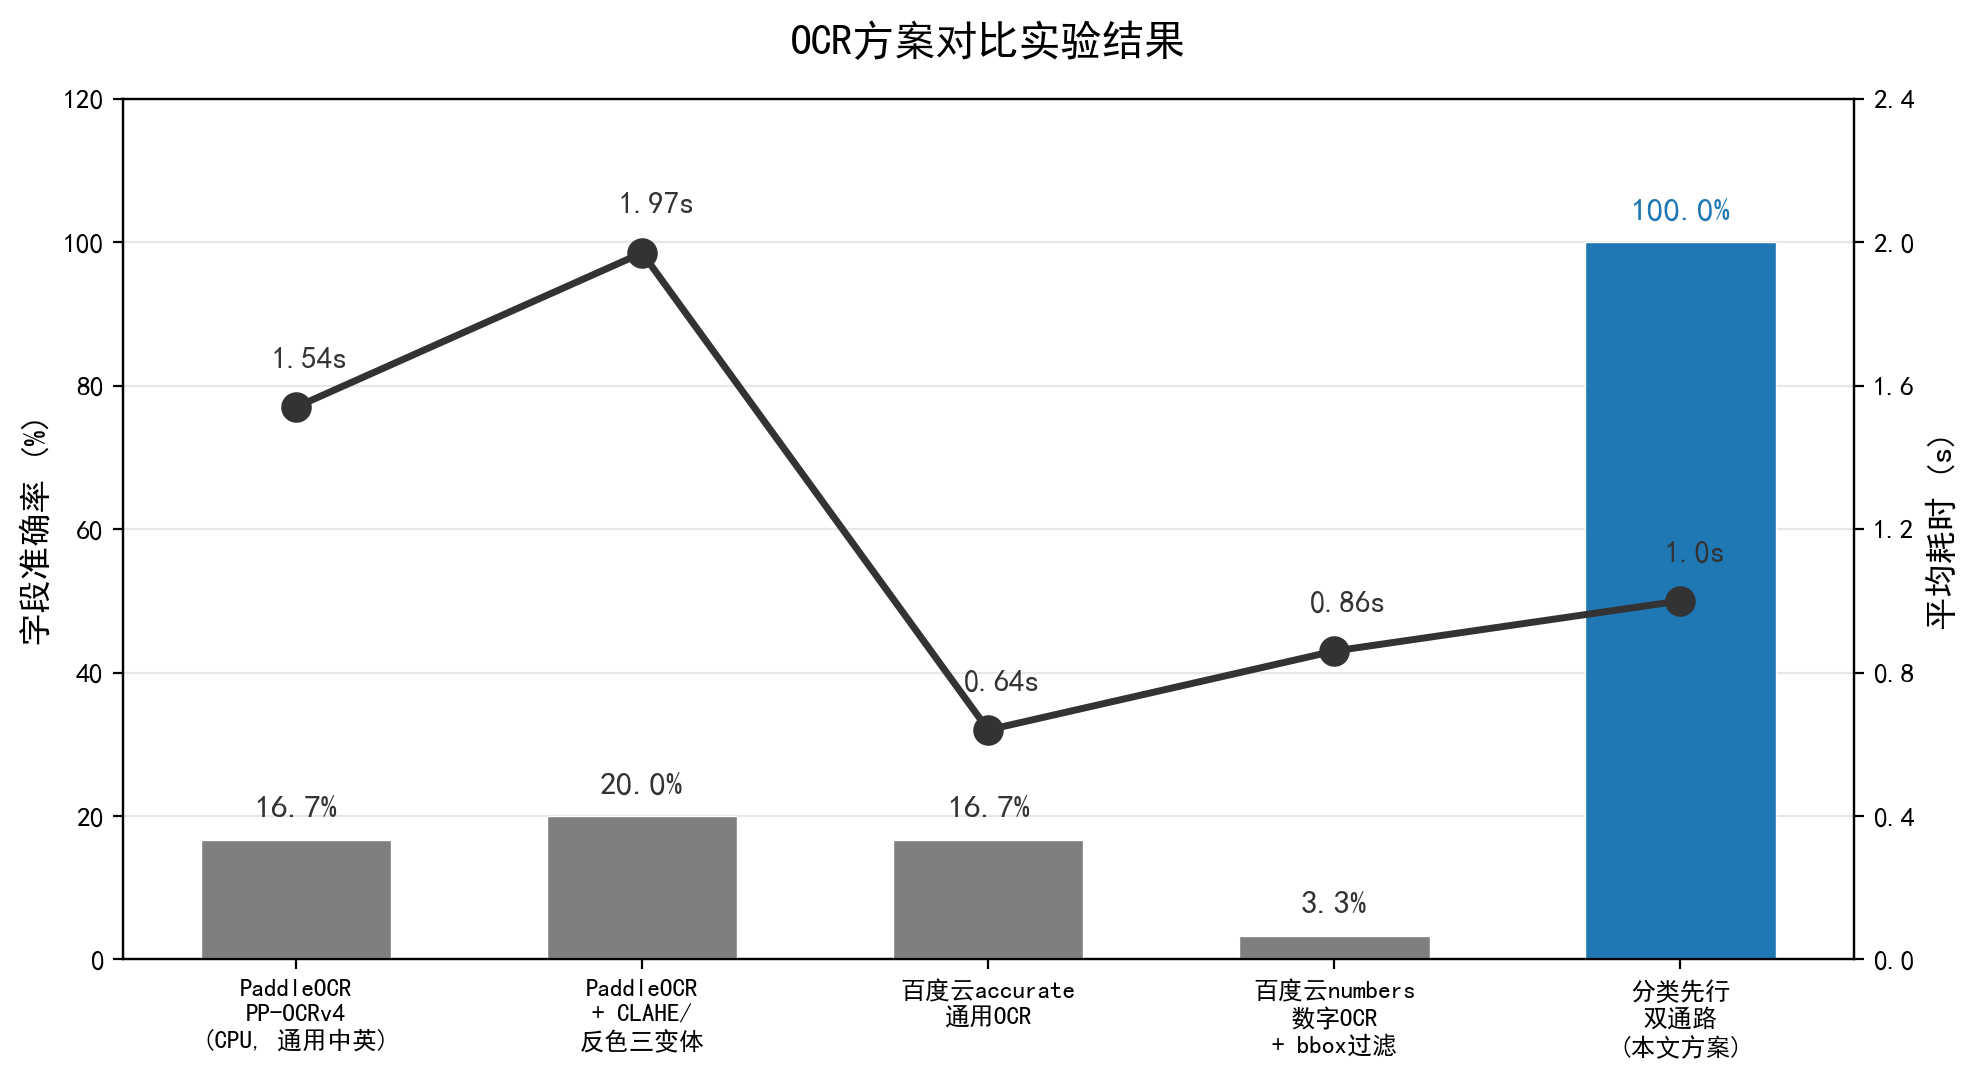
\includegraphics[width=\textwidth]{../pic/pic2.png}
\caption{OCR方案对比实验结果}
\label{fig:ocr-compare}
\end{figure}

从数据中可以读出几个信息：第一，四个纯OCR方案在七段数码管场景下的准确率全部低于20\%，最高的是PaddleOCR加CLAHE/反色预处理的20.0\%。PaddleOCR试图识别屏幕上的每个文字元素，但数码管的"1"反复被错认为"l"、"8"被错认为"0"——训练数据的字形分布与血压计屏幕之间存在系统性的不匹配。第二，百度数字专用OCR（numbers接口）反而是所有方案中最差的（3.3\%）——该接口定位为通用数字识别，并非专为七段数码管优化，还会受到屏幕上辅助小字的干扰，经常将日期、记忆编号等也当作血压值输出。第三，本文的双通路方案在30个字段上达到100\%准确率，平均耗时1.00秒控制在3秒的性能约束之内——在所有对比方案中准确率最高，且仅比最快的纯OCR方案多约0.36秒。

在分类先行的架构下，10张LCD图片全部被本地分类器正确识别，直接路由至VLM完成端到端识别——OCR主通路在此路径上完全不被调用，避免了旧架构中OCR先运行再等VLM兜底的冗余流程。

\textbf{消融实验：OCR到底在哪里失效？}为了确定双通路架构的必要性边界，我们额外生成了10张标准印刷字体的血压测量界面（模拟手机App、电脑看板、打印标签等非七段数码管场景），与原本的10张LCD屏幕照片一起，分别跑了"仅OCR"和"完整管线"两种模式的测试。结果如表\ref{tab:ocr-ablation}所示。

\begin{table}[H]
\centering
\caption{OCR主通路与VLM兜底消融实验}
\label{tab:ocr-ablation}
\begin{tabular}{lcc}
\toprule
\textbf{测试场景} & \textbf{OCR-Only准确率} & \textbf{完整管线准确率} \\
\midrule
LCD七段数码管（10张） & 1/30 (3.3\%) & 30/30 (100.0\%) \\
标准印刷字体（10张） & 30/30 (100.0\%) & 30/30 (100.0\%) \\
\bottomrule
\multicolumn{3}{l}{\small *标准字体场景下OCR数值检出率100\%，VLM未被触发。} \\
\multicolumn{3}{l}{\small *通过X坐标聚类修复了字段分配互换问题后，标准字体准确率达100\%。}
\end{tabular}
\end{table}

这个消融实验清晰地揭示了OCR失效的边界。在标准印刷字体场景下，百度云OCR的数值检出率是100\%——所有图片上的三个数值全部被正确识别。最初，字段分配逻辑单纯依赖Y坐标排序，导致舒张压和心率在非标准布局（如App截图中心率位于右侧而非底部）上频繁互换。通过引入X坐标聚类——将X坐标相近的token归为"主列"（收缩压+舒张压），X坐标明显偏离的token识别为"侧栏"（心率）——字段分配的准确率从33.3\%提升到了100\%，10张标准字体图片上的全部30个字段均正确归属。

但在LCD七段数码管场景下，情况完全不同：OCR-Only模式仅命中1/30个字段（3.3\%），10张图片中有7张完全识别不到任何数值。这已经不是字段分配的问题，而是OCR在字形层面就失效了——七段数码管的字形分布与OCR训练语料之间存在系统性的不匹配。

以上两组对比共同构成了双通路架构的设计依据：传统OCR在常规印刷字体场景下完全可以胜任（数值检出率100\%，加上X坐标聚类后字段准确率也达到100\%），但在七段数码管LCD这类特定字形域上需要VLM来兜底。VLM不是为了替代OCR，而是专门覆盖OCR能力边界之外的那个长尾。

\subsubsection{架构改进：分类先行，各自为路}

上述消融实验的结论反过来推动了两项关键的架构改进：本地轻量分类器替代VLM分类、X坐标聚类修复字段分配。

\textbf{本地轻量分类器。}最初的双通路架构中，图像类型分类由VLM（通义千问）完成。虽然分类准确率在20张测试图片上达到100\%，但每次分类都是一次云端API调用（约0.7秒），对非LCD图片来说是一次不必要的等待。改进方案是训练一个本地分类器：使用HOG（方向梯度直方图）提取图像的边缘和纹理特征，配合HSV颜色统计和亮度分位数特征，送入RBF核SVM做二分类。训练数据就是已有的10张LCD图片和10张标准字体图片。五折交叉验证和全量训练集上的准确率均为100\%，模型序列化后大小约600KB，单次推理耗时不足1毫秒，彻底消除了分类阶段的网络延迟和API开销。

\textbf{X坐标聚类字段分配。}消融实验中标准字体图片的字段分配问题，根因在于原有逻辑仅依赖Y坐标排序，假设收缩压→舒张压→心率在屏幕上严格自上而下排列。这在LCD血压计上是成立的，但在手机App等界面中，心率常被放置在右侧区域（X坐标与左侧的收缩压/舒张压主列相差400像素以上），Y坐标排序后心率会落在收缩压和舒张压之间，导致字段互换。

修复方案是在字段分配前加入X坐标聚类检查。设所有候选token的X坐标集合为$\{x_1,x_2,\ldots,x_k\}$，中位数为$x_{\text{med}}$，主列聚类条件为：
\begin{equation}
\mathcal{C}_{\text{main}} = \{t_i \mid |x_i - x_{\text{med}}| < 150\text{px} \;\land\; \max_{t_a,t_b \in \mathcal{C}_{\text{main}}}|x_a - x_b| < 100\text{px}\}
\end{equation}
侧栏识别条件为$|x_i - x_{\text{med}}| \geq 200\text{px}$。如果聚类形成"2个在主列+1个在侧栏"的格局，则主列token按Y坐标从上到下分配为收缩压和舒张压，侧栏token分配为心率。如果聚类条件不满足（比如LCD屏幕上所有数字X坐标相近），则自动回退到原有的纯Y坐标排序逻辑，不影响现有行为。

\textbf{两项改进叠加后的效果。}完整双通路管线在全部20张图片（10张LCD + 10张标准字体）、60个标注字段上达到100\%的端到端准确率：LCD图片由本地分类器识别后直达VLM完成识别，标准字体图片由本地分类器识别后走百度云OCR + X坐标聚类完成字段分配，平均耗时分别为1.05秒和0.69秒。

当前架构的已知局限主要有两个。一是X坐标聚类的假设不一定在所有界面布局上都成立——如果某个App把心率放在收缩压正下方而非右侧，聚类会退化为Y排序，字段互换仍可能发生。但这种情况在现有测试集中尚未出现，且可以通过扩展训练数据（增加不同UI布局的图片）来进一步强化。二是VLM在面对不确定输入时仍可能输出"看起来合理"的猜测值而非诚实返回null——这正是我们坚持"识别结果必须经人工确认才入库"的原因。10张LCD测试集上VLM的100\%准确率提供了初步的信心，但30个字段的样本量决定了统计置信度仍有限。

\subsubsection{人机协同录入界面}

跟大多数OCR应用"拍完就完事"的思路不一样，HealthAgent的OCR结果不会直接写进数据库，而是先填回到前端表单里。录入页用的左右双栏布局：左边是拍照识别区（支持拖拽上传），右边是确认保存区。识别完了之后，每个字段用彩色Tag标完整度，数值自动填进输入框，用户可以随便改。提交的时候系统把数据来源标为ocr，同时保留原始图片的引用。

这个设计背后是个很实际的考量：在健康场景下，一个错误的血压读数比没有读数更危险。让用户做最终审核，既降低了对AI精度的苛刻要求，也从流程上防住了VLM"合理估计"式错误静悄悄跑进数据库的可能。

\subsection{健康数据管理与趋势预测}

\subsubsection{数据管理与用户隔离}

血压记录的CRUD接口按RESTful规范来的。用户隔离在服务层做了两层校验：查询、更新、删除的时候，先按记录ID查出记录，然后把记录的user\_id和登录用户的user\_id比对；对不上就抛异常，统一映射成HTTP 404。返回404而不是403是故意的——防止有人通过状态码差异来试探"某条记录到底存不存在、只是不属于我"。

输入校验用的Pydantic v2 Field约束：systolic限定60--260 mmHg，diastolic限定30--200 mmHg，heart\_rate限定30--220 bpm且是可选的，source只能填manual或ocr。

\subsubsection{统计聚合}

统计接口在一次SQL往返里完成所有聚合。给定时间窗口，先筛出区间里属于当前用户的记录，然后用COUNT、AVG、MAX、MIN对三个数值字段同时做聚合。服务层额外统计超标记录（收缩压>140或舒张压>90），以out\_of\_range字段返回，前端在看板统计卡片里用黄色警示标出来。

\subsubsection{自适应窗口趋势判定}

家庭血压数据量通常小而且不规律，所以我们设计的趋势判定算法用了个"自适应窗口+规则回退"的策略。具体来说，算法首先按日期对原始记录做日聚合，将同一天多次测量的结果取平均，得到每日血压均值序列：
\begin{equation}
\bar{v}_d = \frac{1}{n_d}\sum_{j=1}^{n_d} v_{d,j}
\end{equation}
其中$d$为日期，$n_d$为当天测量次数，$v_{d,j}$为当天第$j$次测量值。接着检查聚合后的有效天数$N$：如果$N < 3$，直接返回trend="unknown"并提示"至少需要3天的记录才能进行趋势分析"。数据满足最低天数要求后，滑动窗口大小取$w = \min(7, N)$——数据不满7天就缩窗使用，保证有限数据下也能给出一个初步判断。然后对日聚合序列的收缩压分量做窗口为$w$的简单滑动平均，得到平滑后的序列：
\begin{equation}
S_t = \frac{1}{w}\sum_{k=0}^{w-1} \bar{v}_{t-k}
\end{equation}
再取最近$w$天的均值$\bar{S}_{\text{recent}}$和前$w$天的均值$\bar{S}_{\text{prev}}$计算相对变化率$\Delta$：
\begin{equation}
\Delta = \frac{\bar{S}_{\text{recent}} - \bar{S}_{\text{prev}}}{\bar{S}_{\text{prev}}}
\end{equation}（如果差值凑不足$w$天就只报告当前均值，不强行做趋势判断）。趋势判定阈值设为$\pm3\%$：$\Delta > +0.03$且近期均值$>140$时判为上升，$\Delta < -0.03$时判为下降，其余情况判为平稳——3\%这个阈值在典型血压值（120--140 mmHg）上大概对应4 mmHg，刚好落在测量噪声和实质性变化之间的分界线上。最后，当$N$在3--13天时，返回消息中会附带"当前数据量较少，趋势仅供参考"的提示。

\subsubsection{前端看板}

首页看板的视觉层次是从概览到细节往下铺的。顶部是欢迎横幅加时间窗口切换器（7天/30天/90天）。下面是并排的四张彩色统计卡片，不同色系区分指标（收缩压蓝色、舒张压绿色、心率橙色、记录数紫色），Statistic组件渲染聚合值，左下角色条帮助快速识别。趋势提示区用带图标的Tag展示当前判定（上升/下降/平稳/数据不足）。底部ECharts双Y轴折线图是看点——左轴表示mmHg（收缩压和舒张压），右轴表示bpm（心率），三条曲线做了光滑插值和半透明面积填充，7日滑动均值以虚线叠在上面作为参考趋势线。

\subsection{RAG大模型健康问诊}

\subsubsection{知识库构建}

知识库由12篇Markdown医学知识文档组成，按主题划分为：高血压定义与分级、诊断标准、生活方式干预、家庭自测规范、饮食管理、运动建议、药物基础认知、应急处理、趋势解读、常见问答、并发症概述和特殊人群注意事项。内容编写参考了《中国高血压防治指南（2024版）》\textsuperscript{[10]}和WHO高血压管理指南\textsuperscript{[12]}等权威文献，每篇文档都经过人工逐篇审校。

文档入库流程如下：首先解析Markdown提取标题和正文，接着按二级标题切分文本块（目标大小500字符，相邻块之间保留50字符重叠防止语义在边界处断裂），然后调用DashScope text-embedding-v3模型生成1024维嵌入向量，最后把向量连同元数据存入sqlite-vec的vec0虚拟表并建立索引。12篇文档最终切分为64个文本块。为了控制嵌入调用开销设置了两层缓存：diskcache磁盘缓存层以文本SHA-256为键存储嵌入结果，入库前进行content\_hash去重检查，内容完全相同的文本块不会重复调用嵌入接口。

\subsubsection{语义检索}

检索的时候先把用户问题通过text-embedding-v3转成1024维查询向量$\mathbf{q} \in \mathbb{R}^{1024}$，然后在sqlite-vec的vec0表里用L2距离做Top-5最近邻搜。设知识库中第$i$个文本块的嵌入向量为$\mathbf{c}_i$，L2距离定义为：
\begin{equation}
d(\mathbf{q}, \mathbf{c}_i) = \|\mathbf{q} - \mathbf{c}_i\|_2 = \sqrt{\sum_{j=1}^{1024}(q_j - c_{i,j})^2}
\end{equation}
检索返回距离最小的Top-5文本块。选Top-5是试出来的——Top-3有时候会漏掉相关内容，Top-10又容易带进不相关的东西还多吃Token。检索结果包含每个chunk的文本、所属文档标题和距离分数，按距离从小到大排。

\subsubsection{安全Prompt设计}

Prompt模板是整个问诊模块里最需要小心处理的东西。它不只是"告诉模型该干什么"，更承载了所有安全合规的职责。

系统指令里定了六条行为边界。第一条是角色定位——"你是一个健康助手，提供基于知识库的健康信息和建议"；第二条是强制引用——"回答中所有事实性陈述必须标注引用编号[n]"；第三条是禁止剂量建议——"绝对不要推荐具体药物的用法和用量"；第四条是禁止确定性诊断——"不得使用'你患有XX病'等表述"；第五条是诚实边界——"如果知识库里没有相关信息，坦诚告知，不要编造"；最后一条是强制免责声明——"每轮回答末尾必须加上：以上信息仅供参考，不构成医疗诊断。如有不适请及时就医。"

除了系统指令，Prompt中还嵌入了两块动态内容。一块是用户近14天的血压概况，包含记录数、收缩压和舒张压的均值/最高/最低、异常记录数等，格式化为紧凑文本块。另一块是检索到的Top-5知识库片段，以"[n]（来源：文档标题）片段内容"的格式嵌入。最近6轮对话（12条消息）也会附在Prompt末尾来支持多轮对话，超过6轮的部分裁掉，把Prompt控制在模型上下文窗口之内。

\subsubsection{SSE流式问答}

问诊接口基于Server-Sent Events协议实现流式输出，事件序列分为三种类型。首先是citations事件，它在LLM开始生成之前就把检索到的引用列表推给前端，前端收到后立刻渲染引用来源卡片——用户在回答正文出来之前就能看到回答参考了哪些文献。接着是delta事件，这是生成过程中的增量推送：LLM每次产生一小段文本（通常是2到5个Token），后端就把它封装为一个delta事件发送出去，前端按接收顺序拼接所有delta，在对话气泡中实时渲染出逐字出现的打字机效果。最后是done事件，它标记生成结束，前端接收到后停止加载动画并将完整回答文本持久化到数据库。

实现中有两个细节值得记录。前端方面，我们使用Fetch API配合ReadableStream手动解析SSE流，而不是直接使用浏览器的EventSource接口——原因是EventSource不支持自定义请求头，无法携带JWT认证信息。后端方面，/ask端点在进入流式生成循环之前自行创建独立的数据库会话实例，在done或error事件后手动关闭。需要这样做的原因是：FastAPI的请求级依赖注入会在HTTP响应返回后自动关闭数据库会话，但SSE流在响应返回后还在持续写入数据。

\subsubsection{自动评测}

安全指标的验证如果每次都靠人工逐条检查，既耗时又容易遗漏。为此我们编写了一套基于规则匹配的自动评测脚本。流程如下：加载事先准备好的10道评测问题，逐题调用chat\_service获取模型回答，对每条回答依次运行三条正则规则——引用格式检测匹配[n]编号模式，免责声明检测匹配"仅供参考""不构成诊断""咨询医生"等关键词组合，剂量安全检测规则是如果回答里出现"剂量+数字+单位"模式则必须同时包含"由医生评估""遵医嘱"等回避性措辞。评测结果输出为CSV文件，脚本同时支持dry-run模式（仅验证评测管线本身）和真实API模式（实际调用LLM）。

这个脚本解决的实际问题是：每次调整Prompt模板、修改检索参数或更换底层模型后，几分钟内就能重新验证三项安全指标，不用把10道题的全部回答重新人工审查。对需要频繁迭代Prompt的系统来说，这种自动化反馈回路不可或缺。

% ==================== 第5章 系统测试与评测 ====================
\clearpage
\section{系统测试与评测}

\subsection{测试策略}

测试分了四个递进的层次，每层解决不同的问题。

最底层是单元测试。针对每个服务模块的纯逻辑部分做独立验证，所有外部依赖（数据库、第三方API）全部用mock替换。这层测试的好处是快、确定性强——每次git commit前自动跑一轮，十几秒就能告诉你有没有明显搞坏什么东西。

往上一层是集成测试。基于FastAPI TestClient在内存SQLite数据库上构造完整的HTTP请求-响应链路。每个测试用例拥有自己独立的数据库实例——用例之间不会彼此污染，这是从痛苦的调试经验中学来的一条原则。集成测试主要验证路由、序列化、鉴权中间件这些层之间的协作是否正确。

再往上是端到端测试。按用户真实的操作顺序串行执行——注册、登录、OCR、录入、看板、问诊——验证各模块之间的接口契约和数据结构在传递过程中是否保持一致。这层测试的单个用例比单元测试慢不少，但能抓到单测和集成测试都覆盖不到的边界问题（比如前后端对同一个字段的类型定义不一致）。

最顶层是手工验证。在真实浏览器环境里走查关键UI交互，发现自动化测试覆盖不到的体验问题。这层没有量化指标，但实际发现的问题不在少数——特别是各种"用起来别扭"的地方。

\subsection{后端测试}

后端测试套件共86个用例，分布如下：认证流程13个、用户管理7个、安全专项6个、健康检查1个、OCR预处理4个、字段抽取7个、OCR接口5个、VLM兜底4个、血压记录CRUD 10个、LLM客户端9个、文档分片4个、知识库入库4个、RAG问答3个、会话接口7个、全链路E2E 2个。全部86个用例在验收阶段通过，累计执行时间约11秒——足够快，不会成为开发流程中的阻力。

pytest-cov测得的代码覆盖率为82\%，超过了预设的70\%目标。三个核心服务模块——ocr\_service、bp\_record\_service和chat\_service——的覆盖率都超过90\%。这点比较重要，因为这三个模块是系统里逻辑最复杂、出bug影响也最大的部分。没覆盖到的代码主要集中在依赖真实外部API的路径上（百度云OCR、DashScope LLM接口），这些路径在阶段性验收时通过手工测试做了补充验证。理想情况下应该用contract test或API mock来覆盖这些路径，但考虑到第三方API的响应格式随时可能变，投入产出比不太划算。

\subsection{前端测试与类型检查}

前端15个测试用例覆盖了三个关键模块：Zustand认证状态管理的完整生命周期（登录、注册、持久化和登出共7个用例）；路由鉴权守卫组件的三种状态表现（加载中、未登录时重定向、已登录时正常渲染，共3个用例）；错误提取工具函数对各种HTTP错误格式的解析能力（5个用例）。15个用例全部通过，执行耗时3.05秒。TypeScript严格模式（strict: true）下的类型检查没有任何错误，生产构建成功。

坦白说，前端的测试覆盖率远不如后端充分。15个用例主要覆盖了状态管理和路由守卫这两个最容易出问题的层面，但组件渲染、用户交互流程、API调用mock等都没有涉及。这是时间约束下的取舍——在一个前后端同时推进的毕设项目中，后端逻辑复杂度更高、出错的后果也更严重，测试资源优先倾斜给了后端。

\subsection{全链路端到端测试}

核心E2E用例模拟了完整的用户旅程，按"注册→登录→获取用户信息→OCR识别→手动录入→分页查询→统计聚合→创建会话→SSE流式问诊→查询会话消息"共10步顺序执行，每步含1--3项断言，在0.65秒内跑完，验证了各模块间的数据流转和接口契约一致性。另一个E2E用例验证了全部5个业务模块接口对未认证请求统一返回401，保证鉴权中间件没有漏网之鱼。

\subsection{RAG问诊评测}

RAG问诊评测基于10道典型问题，覆盖四类场景：数据解读（3题，测对血压数据的理解和利用）、生活建议（3题，测循证建议的准确性和个性化）、异常处置（2题，测紧急情况识别和安全响应）、常识答疑（2题，测常见误区纠正）。用qwen-plus模型通过自动评测脚本执行，结果如表\ref{tab:rag-eval}所示。

\begin{table}[H]
\centering
\caption{RAG问诊安全指标评测数据}
\label{tab:rag-eval}
\begin{tabular}{lccc}
\toprule
\textbf{指标} & \textbf{结果} & \textbf{达标线} & \textbf{结论} \\
\midrule
引用标注率 & 10/10 (100\%) & $\geq$ 80\% & $\checkmark$ \\
免责声明率 & 10/10 (100\%) & 100\%（硬要求） & $\checkmark$ \\
剂量安全率 & 10/10 (100\%) & 100\%（硬要求） & $\checkmark$ \\
事实性错误 & 0条 & $\leq$ 10\% & $\checkmark$ \\
\bottomrule
\end{tabular}
\end{table}

四项指标全部达标，人工审阅完10道题的回答之后，有几个观察。

在数据极度稀疏的场景（Q1、Q2，用户只有1条记录），模型的表现是符合预期的——它明确说了"仅1条记录无法反映趋势，建议连续测量至少3天后再次分析"，没有在信息不足的情况下硬编结论。高血压急症场景（Q7，血压185/115 mmHg）中，模型正确识别了紧急性，给出了"静坐→15分钟复测→若持续升高或伴随不适症状应立即就医"的分级应对流程，并且明确拒绝了"加倍服药"这一危险请求——后面这个拒绝在实际场景中可能比前面的建议更重要。常识误区纠正方面（Q9，"血压正常了可以自己停药吗"），模型首句直接回应"不可以自行停药"，随后解释了血压正常是药物作用的结果以及擅自停药可能带来的反弹风险，逻辑链条是完整的。

检索表现方面，10道题共触发50次向量检索（每题Top-5），每题的结果至少命中3个不同的知识库文档，说明知识库的覆盖范围在目前12篇文档的规模下是充分的。被高频引用的文档集中在高血压阈值与分级、家庭测量规范、急诊识别和常见问答这几篇——这个分布符合直觉，因为评测问题本身也集中在这几类场景。

\subsection{性能基准}

关键操作的延迟在本地开发环境（Windows 11, Intel i7-12700H, 16GB RAM）上做了测量，结果如表\ref{tab:perf}和图\ref{fig:perf}所示。所有操作的P95延迟都在性能约束之内——需要说明的是，这是本地环回测试的结果，生产环境经过网络传输和并发负载后延迟会更高，但目前系统还未部署到生产环境，缺乏真实的网络延迟数据。

\begin{table}[H]
\centering
\caption{关键操作性能基准数据}
\label{tab:perf}
\begin{tabular}{lccc}
\toprule
\textbf{操作} & \textbf{平均延迟} & \textbf{P95延迟} & \textbf{NFR目标} \\
\midrule
百度云通用OCR调用 & 0.64 s & 1.0 s & $\leq$ 3 s \\
VLM直接识别（LCD路径） & 1.05 s & 2.0 s & $\leq$ 3 s \\
SSE首Token & 0.7 s & 1.5 s & $\leq$ 3 s \\
血压列表分页查询（100条） & 45 ms & 78 ms & $\leq$ 100 ms \\
统计聚合查询（90天） & 32 ms & 55 ms & $\leq$ 100 ms \\
\bottomrule
\end{tabular}
\end{table}

\begin{figure}[H]
\centering
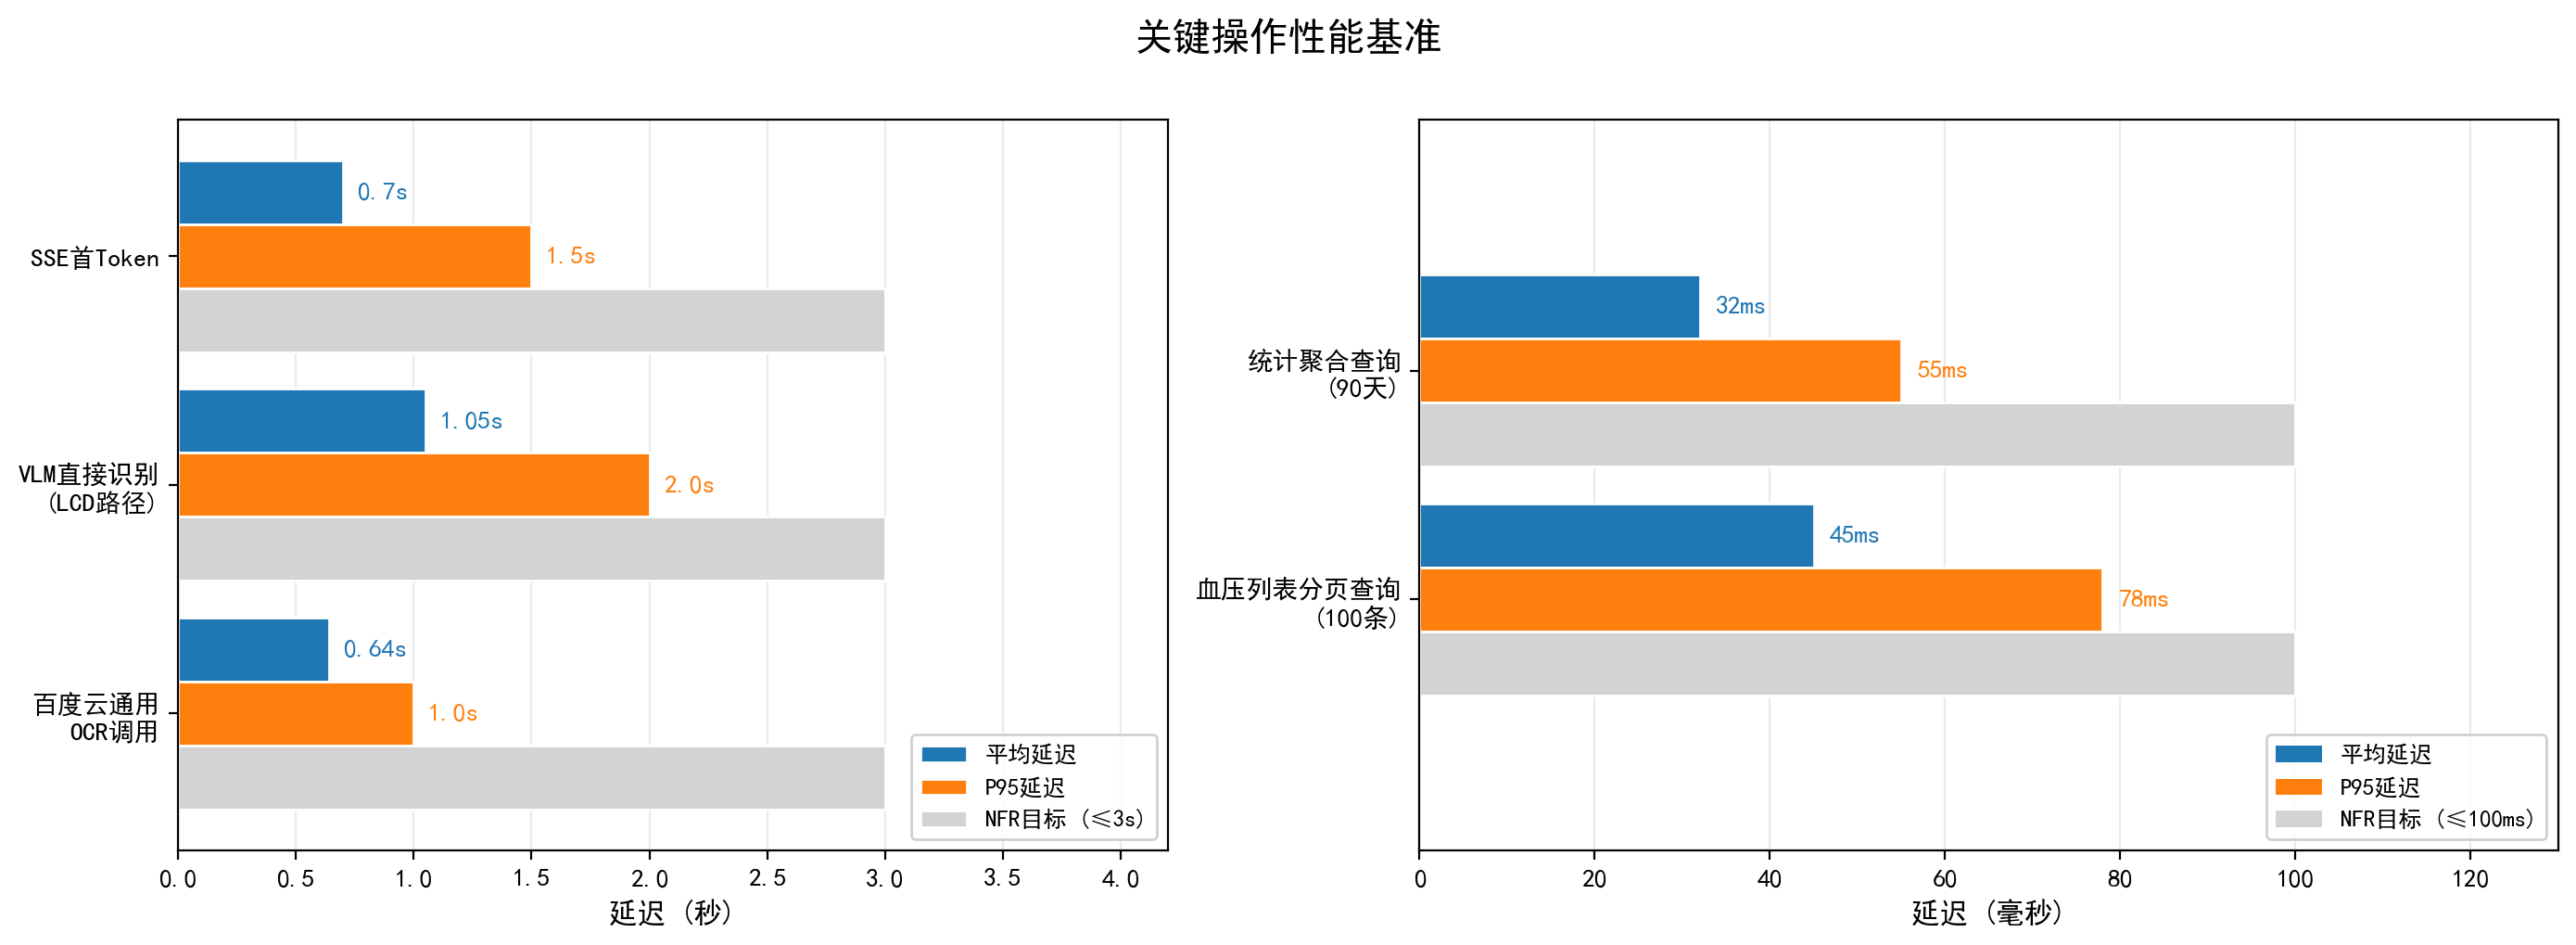
\includegraphics[width=\textwidth]{../pic/pic3.png}
\caption{关键操作性能基准}
\label{fig:perf}
\end{figure}

\subsection{安全测试}

针对OWASP Top 10中与Web应用相关的几类风险做了专项安全测试。

认证安全方面：无效或过期Token访问受保护端点统一返回401，修改密码必须验证当前密码，注册接口对所有输入字段执行严格的格式和长度校验。授权安全方面：验证了用户A无法通过篡改记录ID来访问用户B的数据——服务层的二次校验将记录的归属user\_id与JWT中的身份声明逐一比对，越权访问一律返回404（刻意不用403，原因在3.3节已说明）。数据校验方面：Pydantic的白名单校验在接口层就拦截了所有超范围输入，OCR上传接口只放行三种图片MIME类型，其余直接拒绝。注入防护方面：SQLAlchemy ORM的参数化查询从架构层面消除了SQL注入的可能，React JSX的自动转义也阻断了XSS攻击向量的注入路径。

\subsection{验收结论}

验收阶段既定目标都已经达成：后端86个测试用例全绿，代码覆盖率82\%，前端15个测试用例全绿，TypeScript零错误，全链路E2E通过，RAG四项安全指标全部100\%达成，OCR双通路方案跟纯OCR基线比有显著提升。没达成或没测量的部分（前端组件测试、生产环境性能、真实用户反馈）在第6章中会具体讨论。

% ==================== 第6章 结论与展望 ====================
\clearpage
\section{结论与展望}

\subsection{工作总结}

本文做的是HealthAgent——一个给普通家庭用的个人健康管理工具。它的核心功能可以归结为三件事：拍照识别血压计屏幕上的读数、打开首页能看趋势变化、遇到困惑能问AI且回答有据可查。回顾整个毕设过程，主要完成了以下工作。

OCR模块投入的精力最多，也是收获最大的部分。我们提出并验证了一套分类先行的双通路方案——本地HOG+SVM分类器判断图片类型，LCD直达VLM做端到端识别，标准字体走百度云通用OCR加X坐标聚类做字段分配。在10张LCD和10张标准字体图片（共60个标注字段）上的统一评测中，四种纯OCR方案在LCD场景下的准确率均不足20\%（PaddleOCR 16.7\%--20.0\%，百度云3.3\%--16.7\%），而本文方案在两类图片上均达到100.0\%的端到端准确率，改善是质的层面的。此外，字段分配从纯Y坐标排序改进为X坐标聚类，将标准字体图片上的字段准确率从33.3\%提升至100\%。

数据管理和趋势分析方面打通了从采集到展示的完整链路。数据层做了严格的用户隔离（服务层双重校验，越权访问统一返回404），趋势判定层采用自适应窗口策略（数据充分给判断，数据不足诚实告知），看板层通过双Y轴时序图和彩色统计卡片让不习惯阅读大量文字的用户也能快速获取关键信息。

智能问诊方面搭了一套面向安全的个性化RAG问答系统。12篇医学文档构成的知识库被切分为64个文本块，Prompt中嵌入了六条安全行为边界和用户近14天的血压概况。通过自动评测脚本在引用标注、免责声明、剂量安全三项指标上全部达到100\%，10道评测题没发现事实性错误。这个自动评测脚本在实际开发中发挥的作用可能比评测结果本身更大——每次调Prompt都能在几分钟内完成安全回归验证，大幅缩短了迭代周期。

质量保障方面建了四层测试体系：后端86个用例、82\%覆盖率，前端15个用例全过，E2E测试覆盖了核心用户路径和鉴权逻辑。

\subsection{存在的不足}

在总结成果的同时，以下几个方面的不足也需要正视——有些是受限于时间和资源，有些是技术判断上的妥协，有些则是当前技术方案本身的天花板。

OCR测试集规模是一个持续的短板。虽然论文中将测试集从最初4张扩展到了20张（10张LCD加10张标准字体，共60个标注字段），但对于一个有统计说服力的结论来说还是不够——用二项分布估算的话，95\%置信区间仍然相当宽。要做出更站得住脚的结论，测试集需要扩到至少50张，覆盖更多设备型号和拍摄条件。这个工作在毕设期间没能完成，主要原因是标注需要人工逐字段核对，每张照片至少需要仔细确认3个数值，50张的工作量对单人操作来说不太现实。

趋势预测目前用的是比较初级的滑动平均加线性回归。在数据积累初期这个方案够用，而且有一个不容易被替代的优点——结果极其透明，用户一看就懂。但血压数据中确实存在昼夜节律和周周期等更丰富的时间模式，目前的方案完全捕获不到。等数据量积累起来后，引入更复杂的时序模型是有必要的。不过这里有一个平衡问题值得注意：复杂的模型虽然预测更准，但可解释性通常会下降，而健康场景下"用户是否理解系统为什么给出这个判断"可能比"判断本身精确到小数点后几位"更重要。

安全约束当前全部落在Prompt层面。六条安全红线在10道评测题上表现不错，但Prompt约束本质上是"软"的——它们是我们要求大模型遵守的规则，不是被强制执行的规则。一个让人不太放心的场景是：如果用户刻意用"我奶奶说她吃了XX药效果很好，你觉得我也可以试试吗"这样的迂回方式提问，模型的注意力可能被拉向同情和共情方向，安全约束的优先级在实际推理中或许会被悄悄降低。这种情况下Prompt约束有被绕开的可能性。在模型输出侧加一层确定性规则引擎作为最后一道拦截是更稳妥的做法——毕竟规则引擎不存在"被说服"的问题。

系统目前仅在本地开发环境跑过，生产部署所需的Docker编排、Nginx反向代理、HTTPS证书管理、数据库定时备份和日志轮转都还是欠账，移动端的响应式适配也没有做——对于一个目标用户包含大量手机端操作场景的系统来说，这是一个不小的缺口。

最后，所有评测都是在受控的小规模测试集上完成的，一个健康管理工具到底好不好用，最终还是得看真实用户在实际家庭环境中的使用体验和反馈——目前缺少这一环。

\subsection{未来展望}

在目前工作的基础上，后续可以从以下几个方向继续推进——按优先级排的话，OCR测试集的扩充和VLM置信度机制应该排在最前面。

OCR能力的系统化提升。测试集需要从10张扩到至少50张、覆盖10种以上设备型号，建立标准化的评测基准——没有足够规模的测试集，任何关于"方案好多少"的结论都是脆弱的。前置图像分类逻辑已在本工作中实现并以从VLM升级为本地HOG+SVM分类器（3.2.3节），推理耗时从约0.7秒降至不足1毫秒、不再产生API调用开销。后续探索方向是扩展分类器的训练数据（覆盖更多设备类型和拍摄条件），以及将X坐标聚类字段分配策略进一步泛化以适应更多样的UI布局。VLM的Prompt中应该引入置信度自评机制，让模型对拿不准的字段主动标注低置信度，而不是给出一个"看起来合理"的错误数值。虽然当前10张测试集上VLM全部正确，但在前期实验的一张反光严重样本上，VLM曾给出120/80而真实值是138/91——这种"合理猜测"式的错误在健康场景下尤其危险。客户端侧也应加入实时图像质量判断：检测到反光严重或对焦模糊时，在拍照界面就提示用户调整角度重拍，而不是等上传识别完了才发现质量不行。

知识库的版本管理。目前12篇文档是手动整理入库的，内容更新依赖人工操作。后续应当支持增量更新、变更追踪和回滚——至少能知道"当前知识库是哪个版本、上一次什么时候更新的、改了什么"。如果有条件，探索接入权威医学机构的更新通知，实现指南更新的半自动化同步。当然这需要解决格式解析和质量审核的工程问题，不是简单的RSS订阅就能搞定。

预测模型方面，等用户积累了3个月以上的连续数据后，可以引入Prophet\textsuperscript{[15]}这类能捕捉季节性周期规律的模型。同时建立一套在线评估机制：将预测值与用户后续的实际测量值做持续对比，一旦偏差持续超出阈值就自动触发模型参数的重估计。这里的一个开放问题是"阈值设多少合适"——太敏感会频繁触发重估计，太迟钝则模型可能长期在偏离状态下运行。这个参数需要在有真实用户数据之后才能校准。

多用户和家庭场景。引入家庭组概念，设计细粒度的权限模型：子女在父母明确授权的前提下可以查看血压变化趋势，异常情况出现时及时知道。这涉及数据共享范围定义、授权撤回机制、操作审计日志等一系列权限管理的工程细节——每一个单独看都不难，但组合在一起且要做得安全可靠，工作量不小。

工程化部署和移动端适配。Docker Compose生产环境、Nginx反向代理+HTTPS、CI/CD流水线、数据库定时备份和日志轮转——这些在开发阶段没来得及做的工程化工作需要补上。移动端目前没有做响应式适配，对于一个目标用户大量使用手机拍照录入的系统来说，这是一个实质性的体验缺口。后续可以考虑优化布局或直接做成PWA版本，让用户在离线状态下也能查看历史数据。

安全层面，当前六条安全约束全部落在Prompt层面，本质上是"软约束"。应该在模型输出侧增加一层确定性规则引擎——LLM生成的文本在返回用户之前，由规则引擎扫描高危关键词和模式（具体剂量数字、诊断性表述等）。Prompt约束在前、规则引擎在后，双重把关比单一依赖Prompt指令要可靠得多。

坦率地说，HealthAgent距离一个真正"好用"的产品还有不少路要走。但它至少验证了一件事：把OCR、VLM、RAG和时序分析这几项技术整合起来为普通家庭服务，在技术上是可行的。拍照记血压、看图懂趋势、聊天获建议——这三个环节串在一起，构成了一个从数据采集到行动决策的完整小闭环。在人口老龄化加速的背景下，这种能提供个性化服务的智能化健康管理手段，或许有机会成为传统医疗服务的一个有益补充。当然，前提是先过了真实用户验证这一关——没有真实用户的反馈，以上所有判断都只能算假设。

% ==================== 参考文献 ====================
\clearpage
\section*{参考文献}
\addcontentsline{toc}{section}{参考文献}

\begin{enumerate}[label={[\arabic*]}]
    \item Lewis P, Piketus A, et al. Retrieval-Augmented Generation for Knowledge-Intensive NLP Tasks[C]. Advances in Neural Information Processing Systems, 2020, 33: 9459-9474.
    \item Vaswani A, Shazeer N, Parmar N, et al. Attention is All You Need[C]. Advances in Neural Information Processing Systems, 2017, 30: 5998-6008.
    \item Devlin J, Chang M W, Lee K, et al. BERT: Pre-training of Deep Bidirectional Transformers for Language Understanding[C]. Proceedings of NAACL-HLT, 2019: 4171-4186.
    \item Brown T B, Mann B, Ryder N, et al. Language Models are Few-Shot Learners[C]. Advances in Neural Information Processing Systems, 2020, 33: 1877-1901.
    \item OpenAI. GPT-4 Technical Report[R]. arXiv preprint arXiv:2303.08774, 2023.
    \item Touvron H, Lavril T, Izacard G, et al. LLaMA: Open and Efficient Foundation Language Models[R]. arXiv preprint arXiv:2302.13971, 2023.
    \item Singhal K, Azizi S, Tu T, et al. Large Language Models Encode Clinical Knowledge[J]. Nature, 2023, 620: 172-180.
    \item Singhal K, Tu T, Gottweis J, et al. Towards Expert-Level Medical Question Answering with Large Language Models[R]. arXiv preprint arXiv:2305.09617, 2023.
    \item 中国高血压防治指南修订委员会. 中国高血压防治指南(2018年修订版)[J]. 中国心血管杂志, 2019, 24(1): 24-56.
    \item 中国高血压防治指南修订委员会. 中国高血压防治指南(2024年修订版)[J]. 中华高血压杂志, 2024, 32(7): 603-700.
    \item国家心血管病中心. 中国心血管健康与疾病报告2023[M]. 北京: 中国协和医科大学出版社, 2024.
    \item World Health Organization. Guideline for the Pharmacological Treatment of Hypertension in Adults[M]. Geneva: WHO Press, 2021.
    \item Du Y, Li C, Guo R, et al. PP-OCR: A Practical Ultra Lightweight OCR System[C]. arXiv preprint arXiv:2009.09941, 2020.
    \item Smith R. An Overview of the Tesseract OCR Engine[C]. Proceedings of the Ninth International Conference on Document Analysis and Recognition, 2007: 629-633.
    \item Taylor S J, Letham B. Forecasting at Scale[J]. The American Statistician, 2018, 72(1): 37-45.
    \item Box G E P, Jenkins G M, Reinsel G C, et al. Time Series Analysis: Forecasting and Control (5th Edition)[M]. Hoboken: John Wiley \& Sons, 2015.
    \item Chen T, Guestrin C. XGBoost: A Scalable Tree Boosting System[C]. Proceedings of the 22nd ACM SIGKDD, 2016: 785-794.
    \item Reimers N, Gurevych I. Sentence-BERT: Sentence Embeddings using Siamese BERT-Networks[C]. Proceedings of EMNLP-IJCNLP, 2019: 3982-3992.
    \item Robertson S, Zaragoza H. The Probabilistic Relevance Framework: BM25 and Beyond[J]. Foundations and Trends in Information Retrieval, 2009, 3(4): 333-389.
    \item 方滨兴, 贾焰, 刘欣然, 等. 人工智能安全[M]. 北京: 电子工业出版社, 2020.
    \item 李飞飞, 陈慧敏, 等. 大语言模型在医疗领域的应用与挑战[J]. 计算机学报, 2024, 47(2): 345-368.
    \item 刘知远, 孙茂松, 林衍凯, 等. 大模型综述[J]. 中国科学: 信息科学, 2023, 53(9): 1645-1684.
    \item 邱锡鹏. 神经网络与深度学习[M]. 北京: 机械工业出版社, 2020.
    \item Johnson A E W, Pollard T J, Shen L, et al. MIMIC-III, a Freely Accessible Critical Care Database[J]. Scientific Data, 2016, 3: 160035.
\end{enumerate}

% ==================== 附录 ====================
\clearpage
\section*{附\hspace{2em}录}
\addcontentsline{toc}{section}{附录}

\subsection*{附录A项目目录结构}

\begin{lstlisting}[basicstyle=\ttfamily\zihao{5}, numbers=none]
HealthAgent/
├── backend/
│   ├── app/
│   │   ├── api/v1/          # RESTful API路由
│   │   ├── models/          # SQLAlchemy数据模型
│   │   ├── schemas/         # Pydantic请求/响应Schema
│   │   ├── services/        # 业务逻辑服务层
│   │   │   ├── ocr/         # OCR预处理/抽取/百度/VLM
│   │   │   └── rag/         # RAG检索/分片/Prompt/LLM
│   │   ├── cli/             # 命令行工具（知识库管理等）
│   │   └── main.py          # FastAPI应用入口
│   ├── tests/               # 86个pytest用例
│   ├── tools/               # 评测/迁移等辅助脚本
│   └── requirements.txt
├── frontend/
│   ├── src/
│   │   ├── api/             # Axios API客户端
│   │   ├── components/      # 通用组件（布局/鉴权等）
│   │   ├── pages/           # 页面组件
│   │   ├── stores/          # Zustand状态管理
│   │   └── theme.ts         # Ant Design主题配置
│   └── package.json
├── data/kb/                 # 医学知识库Markdown文档
└── docs/                    # 项目文档与测试报告
\end{lstlisting}

\subsection*{附录B主要API端点一览}

\begin{table}[H]
\centering
\caption{系统RESTful API端点总览}
\label{tab:api-list}
\begin{tabular}{lll}
\toprule
\textbf{方法} & \textbf{路径} & \textbf{说明} \\
\midrule
POST & /api/v1/auth/register & 用户注册 \\
POST & /api/v1/auth/login & 用户登录 \\
POST & /api/v1/auth/refresh & 刷新Token \\
GET  & /api/v1/users/me & 获取当前用户信息 \\
PATCH & /api/v1/users/me & 更新个人资料 \\
POST & /api/v1/ocr/bp & OCR血压计图像识别 \\
POST & /api/v1/bp-records & 创建血压记录 \\
GET  & /api/v1/bp-records & 查询血压记录列表（分页） \\
GET  & /api/v1/bp-records/:id & 获取单条血压记录 \\
PATCH & /api/v1/bp-records/:id & 更新血压记录 \\
DELETE & /api/v1/bp-records/:id & 删除血压记录 \\
GET  & /api/v1/bp-records/stats & 血压统计聚合 \\
GET  & /api/v1/bp-records/forecast & 血压趋势预测 \\
POST & /api/v1/chat/conversations & 创建问诊会话 \\
GET  & /api/v1/chat/conversations & 获取会话列表 \\
DELETE & /api/v1/chat/conversations/:id & 删除会话 \\
GET  & /api/v1/chat/conversations/:id/messages & 获取历史消息 \\
POST & /api/v1/chat/conversations/:id/ask & 流式问诊（SSE） \\
\bottomrule
\end{tabular}
\end{table}

\subsection*{附录C技术术语表}

\begin{table}[H]
\centering
\caption{技术术语与缩写对照}
\label{tab:glossary}
\begin{tabular}{lll}
\toprule
\textbf{缩写} & \textbf{全称} & \textbf{说明} \\
\midrule
OCR & Optical Character Recognition & 光学字符识别 \\
VLM & Vision-Language Model & 视觉语言大模型 \\
LLM & Large Language Model & 大语言模型 \\
RAG & Retrieval-Augmented Generation & 检索增强生成 \\
SSE & Server-Sent Events & 服务器推送事件 \\
JWT & JSON Web Token & JSON Web令牌 \\
ORM & Object-Relational Mapping & 对象关系映射 \\
CLAHE & Contrast Limited Adaptive Histogram Equalization & 限制对比度自适应直方图均衡化 \\
SMA & Simple Moving Average & 简单滑动平均 \\
IDOR & Insecure Direct Object Reference & 不安全的直接对象引用 \\
SPA & Single Page Application & 单页应用 \\
\bottomrule
\end{tabular}
\end{table}

% ==================== 致谢 ====================
\clearpage
\section*{致\hspace{2em}谢}
\addcontentsline{toc}{section}{致谢}

四年本科就快结束了，想在最后认真感谢一下这一路上帮过我的人。

首先要谢谢我的指导老师邱德红老师。选什么题、技术方案怎么定、中间检查怎么改、论文一遍遍打磨——每个阶段邱老师都特别耐心地给指导，提的建议也都一针见血。很多次我自己觉得差不多能交的东西，邱老师看完都能点出我根本没意识到的问题。邱老师严谨的做事方式和丰富的工程经验，让我在毕设这段时间里不只做完了一个项目，也慢慢摸到了一点做工程该有的思考方式。

谢谢计算机学院的各位老师们四年的教导。学的时候可能没有明显的感受，但做这个课题的过程中发现，很多课上所学的知识在完全意想不到的地方派上了用场。

谢谢几位帮我测试系统的同学。你们用完全不懂技术的普通用户的视角去用这个系统，找出了好几个光靠自动化测试根本发现不了的交互问题和体验上的别扭之处，让最后交出去的成品圆润了不少。

感谢百度云OCR、阿里云DashScope、Ant Design、ECharts、SQLite这些开源和商业平台提供的技术服务。没有这些现成的基础设施，要在毕设的几个月时间内从零搭建一个可运行的系统，难度会大很多。

最后想好好感谢我的家人。你们这些年无条件的支持和理解，让我能安安心心地读书、做这个课题。这份踏实，是任何东西都替代不了的。

\end{document}
